%%--------------------------------------------------
%%
%% Disserta��o de Mestrado
%% Autor: Bruno Luna - Data(In�cio): 29/11/2010 
%%                     Data(Defesa): 27/02/2012
%%---------------------------------------------------
\documentclass[pt,oneside,onehalfspacing]{risethesis}

%%%%%%%%%%%%%%%%%%%%%%%%%%%%%%%%%%%%%%%%%%%%%%%%%%%%%%%%%%%%%%%%%%%%%%%%
%% PACKAGES AND CUSTOMIZATIONS
%%%%%%%%%%%%%%%%%%%%%%%%%%%%%%%%%%%%%%%%%%%%%%%%%%%%%%%%%%%%%%%%%%%%%%%%
\usepackage{natbib}
\usepackage{babel}
\usepackage{supertabular}
\usepackage{subfigure}
\usepackage{fancybox}
\usepackage{acronym}
\usepackage{url}
% Command to draw lines
\usepackage{tikz}
% Commands for list of symbols
\usepackage[intoc,portuguese]{nomencl}
\makenomenclature
\renewcommand{\nomname}{Lista de S�mbolos}
% Commands for code listings
\usepackage{codehighlight}
\usepackage{minted}
\usemintedstyle{tango}
\newminted{xml}{bgcolor=yellow!10, frame=single, rulecolor=\color{black!50}, label="XML"}
\newminted{python}{bgcolor=yellow!10, frame=single, rulecolor=\color{black!50}, label="Python"}
\renewcommand\listingscaption{Listagem}
%% Change the following pdf author attribute name to your name.
\usepackage{float}
\usepackage[linkcolor=black,citecolor=black,urlcolor=black,colorlinks,pdfpagelabels,pdftitle={brunoluna-msc},pdfauthor={Bruno Gustavo Borges Luna}]{hyperref}
% Command added to present problem in 'theorem form'
\newtheorem{problem}{Problema}
% Definition for tensors format
\def\mathbi#1{\textbf{\em #1}}
% Command for algorithms in pseudocode
\usepackage{algorithm}
\usepackage{algorithmic}

%%%%%%%%%%%%%%%%%%%%%%%%%%%%%%%%%%%%%%%%%%%%%%%%%%%%%%%%%%%%%%%%%%%%%%%%
%% FRONT MATTER
%%%%%%%%%%%%%%%%%%%%%%%%%%%%%%%%%%%%%%%%%%%%%%%%%%%%%%%%%%%%%%%%%%%%%%%%
\address{Recife}

\universitypt{Universidade Federal de Pernambuco}
\universityen{Federal University of Pernambuco}

\departmentpt{Centro de Tecnologia e Geoci�ncias}
\departmenten{Centre for Technology and Geosciences}

\programpt{P�s-gradua��o em Engenharia Mec�nica}
\programen{Graduate in Mechanical Engineering}

\majorfieldpt{Engenharia Mec�nica}
\majorfielden{Mechanical Engineering}

\title{Modelagem Autom�tica de Escoamentos em Meios Porosos via M�todo dos Elementos Finitos}
\date{Fevereiro de 2012}

\author{Bruno Gustavo Borges Luna}
\adviser{Paulo Roberto Maciel Lyra}
\coadviser{Ramiro Brito Willmersdorf}

\begin{document}

\frontmatter
\frontpage
\presentationpage

%SIGNATURES
\newpage
\thispagestyle{empty}
\begin{center}
	\begin{Large}
		Modelagem Autom�tica de Escoamentos em Meios Porosos via M�todo dos Elementos Finitos
	\end{Large}
	
	\begin{large}
		\vfill		
		\emph{Bruno Gustavo Borges Luna}
		\vfill
	\end{large}
\end{center}

Trabalho apresentado ao Programa de P�s-gradua��o em
Engenharia Mec�nica do Centro de Tecnologia e Geoci�ncias
da Universidade Federal de Pernambuco como requisito
parcial para obten��o do grau de Mestre em Engenharia
Mec�nica.

\vfill

Aprovada por:
    
\begin{flushright}
		\tikz\draw (0,0) -- (9,0);\\
		Paulo Roberto Maciel Lyra, Ph.D.\\
		(Orientador)\\
		\vfill
        \tikz\draw (0,0) -- (9,0);\\
		Ramiro Brito Willmersdorf, Ph.D.\\
		(Co-Orientador)\\
		\vfill
		\tikz\draw (0,0) -- (9,0);\\
		Darlan Karlo Elis�rio de Carvalho, D.Sc.\\
		(Examinador Interno)\\
		\vfill
		\tikz\draw (0,0) -- (9,0);\\
		Alessandro Rom�rio Echevarria Antunes, D.Sc.\\
		(Examinador Externo: CAA-UFPE)\\
		\vfill
		\tikz\draw (0,0) -- (9,0);\\
		�zio da Rocha Ara�jo, D.Sc.\\
		(Examinador Externo: DECIV-UFPE)\\	
\end{flushright}

\begin{center}
	\vfill
	
	\vfill
	Recife, Fevereiro de 2012 
\end{center}

%DEDICATORY
\begin{dedicatory}
Aos meus pais, \\ � minha irm� \\
e � minha esposa
\end{dedicatory}

\acknowledgements
Ao Prof.~Paulo Lyra, cuja mentoria foi fundamental para a minha forma��o como profissional, pela orienta��o, confian�a e apoio inestim�veis desde os tempos de inicia��o cient�fica. Agrade�o especialmente pela amizade e paci�ncia demonstradas ao longo dos anos.

\vspace{3 mm}

\noindent
Ao Prof.~Ramiro Willmersdorf, pelos coment�rios sempre sucintos e pertinentes, e tamb�m por sua memor�vel palestra plen�ria no CILAMCE 2008, cujas ideias influenciaram bastante o rumo tomado neste trabalho.

\vspace{3 mm}

\noindent
Aos professores �zio Ara�jo e Alessandro Antunes, pela participa��o na banca examinadora e pelos coment�rios para melhoria da disserta��o.

\vspace{3 mm}

\noindent
Ao Prof.~Darlan Carvalho, pelas v�rias sugest�es para este trabalho e principalmente por todos os ensinamentos transmitidos ao longo dos anos.

\vspace{3 mm}

\noindent
Aos colegas de LABCOM (Rafael, Adriano, Rodrigo, H�lder, Danilo, Ana Paula, etc.), pelos momentos de trabalho e de descontra��o.

\vspace{3 mm}

\noindent
� Petrobras, pelo apoio constante ao grupo PADMEC.

\vspace{3 mm}

\noindent
� minha m�e, Neuce, e ao meu pai, Cosme, aos quais serei eternamente grato pelo apoio incondicional em todos os momentos, pelo incentivo � minha forma��o acad�mica e principalmente por serem os meus maiores orientadores gra�as a todos os valores ensinados atrav�s de exemplos di�rios.

\vspace{3 mm}

\noindent
� minha irm�, Monique, pelo carinho, amizade e por ser sempre um exemplo de dedica��o e vontade.

\vspace{3 mm}

\noindent
� minha esposa, Caroline, por seu amor e por ter estado sempre ao meu lado durante esta jornada. Este trabalho � t�o seu quanto meu. \emph{Ich liebe dich!}

\resumo
A simula��o de escoamentos multif�sicos em meios porosos imp�e v�rios desafios de ordem num�rica devido a uma s�rie de fatores como os meios altamente anisotr�picos e heterog�neos tratados neste tipo de an�lise, as equa��es de natureza acoplada el�ptica-hiperb�lica associadas �s Equa��es Diferencias Parciais (EDP) que descrevem o fen�meno, entre outros. Uma das maiores dificuldades encontradas na simula��o de num�rica de EDPs em geral � a solu��o de grandes sistemas de equa��es lineares. Os m�todos Multigrid permitem obter uma acelera��o de converg�ncia de resolvedores de tais sistemas de equa��es. Entretanto, tais m�todos geralmente exigem uma sequ�ncia de malhas progressivamente menos refinadas, cuja gera��o pode se tornar um problema caso n�o seja adequadamente tratada. Originalmente esta sequ�ncia era constru�da definindo diferentes n�veis de refinamento, manual ou automaticamente, come�ando pela malha mais grosseira. Contudo, esta abordagem frequentemente leva a dificuldades na representa��o de detalhes geom�tricos na malha mais fina. Esta estrat�gia tamb�m pode demandar buscas sucessivas de modo a realizar a interpola��o atrav�s dos diversos n�veis, introduzindo erros adicionais. Uma alternativa para superar estes problemas � a gera��o de toda a hierarquia de malhas de um modo completamente alg�brico utilizando o chamado M�todo Multigrid Alg�brico (AMG). Este trabalho apresenta a implementa��o de um software criado utilizando a ferramenta FEniCS para a gera��o autom�tica de c�digo de baixo-n�vel e PyAMG para a cria��o completamente autom�tica de uma estrutura multin�veis de matrizes que s�o aplicadas na solu��o num�rica de escoamentos em meios porosos usando o M�todo dos Elementos Finitos (MEF). Os m�todos descritos aqui s�o gerais o suficiente para lidar com problemas tridimensionais, heterog�neos e anisotr�picos. Exemplos s�o apresentados e resultados discutidos para problemas bidimensionais com dom�nios homog�neo e heterog�neos com tensores de permeabilidade iso- e anisotr�picos.

\begin{keywords}
Multigrid, Reservat�rio de Petr�leo, Escoamento em Meios Porosos
\end{keywords}

\abstract
The simulation of multiphase flows in porous media imposes many numerical challenges due to a series of factors such as the high anisotropic and heterogeneous media handled in this type of analysis, the Partial Differential Equations (PDEs) with coupled elliptic-hyperbolic mathematical nature, among others. Even after the mathematical and numerical formulations used to model the flow are defined, there is still another challenge regarding the coding of these methods, because it is usually a very time-consuming task to develop computer programs that implement formulations for general and/or complex cases. This work presents the implementation of a software written using the Python programming language and the FEniCS computational tool for the automatic generation of low-level code in C++ applied to the numerical solution of mono- and biphasic flows in porous media using the Finite Element Method (FEM). The classical Galerkin FEM and the Mixed Finite Element Method (MFEM) were tested for the solution of the pressure (pressure and velocity for MFEM) and the Streamline Upwind Petrov Galerkin (SUPG) stabilized FEM with shock capturing operator for the saturation equation. A convergence accelaration technique via Algebraic Multigrid (AMG) was used for the solution of the linear system of equations derived from the Galerkin FEM discretization. The methods described here are general enough to handle three-dimensional, heterogeneous and anisotropic problems. Examples are shown and results discussed for one- and two-dimensional problems in homogenous and heterougenous domains with iso- and anisotropic permeability tensors. The comparisons of the results obtained in this work with those from analytical solutions and literature references show the potential of the developed tool for the simulation of flows in porous media.

\begin{keywords}
Flow in Porous Media, Finite Element Method, Automatic Modelling
\end{keywords}


\tableofcontents
\listoffigures
\listoftables

% ACRONYMS
\chapter*{Lista de Acrônimos}
\addcontentsline{toc}{chapter}{Lista de Acrônimos}
\begin{acronym}
  \acro{MDF}{Método das Diferenças Finitas}
  \acro{MEF}{Método dos Elementos Finitos}
  \acro{MVF}{Método dos Volumes Finitos}
  \acro{UFPE}{Federal University of Pernambuco}
\end{acronym}


\printnomenclature

%%%%%%%%%%%%%%%%%%%%%%%%%%%%%%%%%%%%%%%%%%%%%%%%%%%%%%%%%%%%%%%%%%%%%%%%
%% BEGIN CHAPTERS
%%%%%%%%%%%%%%%%%%%%%%%%%%%%%%%%%%%%%%%%%%%%%%%%%%%%%%%%%%%%%%%%%%%%%%%%
\mainmatter

% CHAPTER 01 - INTRODUCTION
\chapter{Introdu��o}
\label{ch:introduction}

\section{Motiva��o}
\label{sc:motivation}

Nowadays, the numerical simulation of fluid flow in porous media is fundamental in many engineering fields, such as in the analysis of groundwater flow and contaminant transport \citep{Bear1992}, management of water and heat in polymer membranes for fuel cells \citep{Matamoros2006} or for the simulation of multiphase flows in petroleum reservoirs \citep{Peaceman1977, Aziz1979,Ewing1983,Carvalho2005,Silva2008}.

The scientific modeling of fluid flow in porous media for the petroleum industry has been done since the 1930's, initially using sand-packed models to understand the production of water in oil reservoirs and the reason why the water-oil rate increases with time. In the late 1930's and 1940's some experiments with electrolytic models were used to model the flow in porous media, as it was already recognized the analogy between electric current and the Darcy flow \citep{Peaceman1990}. All these physical analogs models allowed a deeper insight in the phenomena governing this kind of problem, but it was not just until the advent of the electronic computers that engineers were able to simulate real-world problems as, for example, that of oil reservoirs in 2 and 3 dimensions. 

Parallel to the development of new hardware, there has been a extensive work on computational methods applied to multiphase flow in porous media. The first method used in large scale for solving partial diffential equations (PDE) numerically and still the standard in the petroleum industry is the finite difference method (FDM) \citep{Peaceman1990}. However, this kind of method presents some disadvantages, as the difficulty to handle complex domains, general boundary conditions or variable material properties \citep{Chen2006}, especially when compared to methods adequate to handle with unstructured meshes that have been applied more recently in this area as the finite volume method (FVM) \citep{Carvalho2005, Cordazzo2006} or the finite element method (FEM) \citep{Chen2006}. For the reasons already cited, the last class of method has been used along this work.

A common aspect among all these computational methods is the considerable amount of time necessary for the development of computer programs that implement formulations for general and/or complex cases. Much of this time is spent coding tasks that are common to almost any numerical simulation software, as for example the matrix assembly, I/O data handling or iterative solutions for linear system of equations. The approach of this work to overcome this difficulty was to use the open source tool \emph{FEniCS/DOLFIN} \citep{Logg2010}, which performs a low-level code (in \emph{C++}),  automatized generation based on some high-level code (in \emph{Python}) input, allowing the developer to focus on developing and testing different mathematical and numerical formulations for the problem of interest using a syntax very similar to the one used for the mathematical description of the problem, instead of spending time writing auxiliary code for ``administrative'' tasks.

Moreover, there is a need to reduce the computing time of the program in order to make the simulations feasible in the time-frame of a project. Normally, the most CPU-time consuming part of a simulation is the solution of the linear equation system resulting from the PDE's discretization with a numerical method \citep{Saad2003}. Meanwhile, several techniques are available to solve iteratively this kind of system, each of them with its own advantages and disadvantages in terms of speed and generality, whereas these mentioned features often lead to distinct directions, that is, a method that is extremely fast for one specific type of problem is not general and vice-versa. In this work, we used one method that is believed to couple almost ideally these two features, namely the Multigrid method \citep{Trottenberg2001, Saad2003, Briggs2000}. Nevertheless, these desired characteristics are not obtained without cost, and in this case the main additional difficulties associated with Multigrid methods are the need of a sequence of progressive coarser meshes whose generation can become an issue if not adequately addressed and the use of operators for data transfer among the successive levels. Following the principle of sparing coding time with general tasks and focusing on the problem of interest, we used in this work the open source library \emph{PyAMG} \citep{Bell2008}, which not only performs in an fully automatic way the matrix-sequence generation given an initial mesh, but also allows the use of many different variants of the Algebraic Multigrid Method (AMG), including the classical Ruge-St\"uben and the Smoothed Aggregation (SA) algorithms \citep{Trottenberg2001}.

\section{Hist�rico da Simula��o de Reservat�rios de Petr�leo}
\label{sc:histSimRes}

\section{Hist�rico do Multigrid}
\label{sc:histMult}

\section{Hist�rico da Modelagem Autom�tica de Equa��es Diferenciais}
\label{sc:histMult}

\section{Objetivos}
\label{sc:obj}

\section{Organiza��o do Trabalho}
\label{sc:orgTrab}




% CHAPTER 02 - MATHEMATICAL FORMULATION
\chapter{Formula��o Matem�tica}
\label{ch:form_mat}

In this work, we have adopted the classical mathematical formulation proposed in \cite{Peaceman1977} for the simultaneous flow of two immiscible phases in a saturated porous medium. This approach has been used by many researchers \citep{Ewing1983,Chavent1986,Carvalho2005,Silva2008} and has as one of its main characteristics the manipulation of the mass conservation equation using the Darcy law to form a system of a parabolic-elliptic pressure and a parabolic-hyperbolic saturation equations \citep{Carvalho2005}, as opposed to other formulations where the pressure and saturation fields are solved simultaneously in a system of parabolic PDEs \citep{Aziz1979}. 
%Describe briefly Aziz's formulation in the thesis, for comparison purposes

The segregated formulation of Peaceman allows the use of specialized methods capable of exploring mathematical characteristics for each equation of the resulting system. The coupling of the two fields is achieved through the use of a total velocity term.

In order to use the equations presented in this section, it is necessary to adopt some simplifying assumptions \citep{Carvalho2005,Peaceman1977}:
\begin{itemize}
\item Totally saturated porous medium;
\item Incompressible fluids and rocks;
\item Immiscible fluids;
\item Isothermal flow;
\item Darcy law valid for the fluids velocities.
\end{itemize}

Considering the assumption of totally saturated porous medium and the existence of $n$ phases, the constitutive equation for saturation yields:
\begin{equation} \label{eq:eq_const_sat}
\sum_{\alpha=1}^n S_{\alpha} = 1
\end{equation}

Where $\alpha$ represents each phase (in this work, $\alpha = w$ and $o$ for water and oil, respectively) and $S_{\alpha}$ represents the saturation of the phase $\alpha$.
% Describe concepts as effective porosity and volume, and then give definition of saturation in the thesis. 
 
The generalized Darcy law for each phase velocity reads as:
\begin{equation} \label{eq:eq_darcy_general}
\vec{v}_{\alpha} = - \frac{K_{\alpha}}{\mu_{\alpha}} \nabla\left(p_{\alpha} - \rho_{\alpha}g\nabla z \right)
\end{equation}
with $K_{\alpha}$, $\mu_{\alpha}$, $p_{\alpha}$ and $\rho_{\alpha}$ represent the effective permeability, viscosity, pressure and density of phase $\alpha$, whereas $g$ and $z$ representing the gravity acceleration and the displacement in its direction, respectively. The relation between the effective  and absolute permeability $K$ accounts for the influence of one fluid on the other during the flow and is defined as the relative permeability:
\begin{equation} \label{eq:relat_perm}
k_{r\alpha} = \frac{K_{\alpha}}{K} \leq 1
\end{equation}
%Cite models for relative permeability (Chen,Aziz as general, Brooks-Corey as specific)

The conservation equation for each phase is described as \citep{Peaceman1977}:
\begin{equation} \label{eq:cons_eq}
-\nabla \cdot \left(\rho_{\alpha} \vec{v}_{\alpha}\right) + q_{\alpha} =
\frac{\partial \left(\phi \rho_{\alpha} S_{\alpha}\right)}{\partial t} 
\end{equation}

The terms $q_{\alpha}$, $\phi$ and $t$ represent sources/sinks of phase $\alpha$ (e.g., wells), effective porosity of rock and time, respectively. Further, if we consider two phases, a wetting (water) and a non-wetting (oil), combining the Eqs. (\ref{eq:eq_darcy_general}) and (\ref{eq:cons_eq}), and using the definition given in Eq. (\ref{eq:relat_perm}), we obtain the following system of partial differential equations which solve the two-phase flow problem under the assumptions taken:
\begin{subequations} \label{eq:twophase_system}
  \begin{equation} \label{eq:twophase_systema}
\nabla \cdot \left(\frac{\rho_{w}Kk_{rw}}{\mu_{w}} \nabla\left(p_{w} - \rho_{w}g\nabla z \right)\right) + q_{w} =
\frac{\partial \left(\phi \rho_{w} S_{w}\right)}{\partial t} 
  \end{equation}
  \begin{equation} \label{eq:twophase_systemb}
\nabla \cdot \left(\frac{\rho_{o}Kk_{ro}}{\mu_{o}} \nabla\left(p_{o} - \rho_{o}g\nabla z \right)\right) + q_{o} =
\frac{\partial \left(\phi \rho_{o} S_{o}\right)}{\partial t} 
  \end{equation}
\end{subequations}
%Stress that these equations are more general then the ones necessary for our assumptions and that they will be simplified

In Eqs. (\ref{eq:twophase_systema}) and (\ref{eq:twophase_systemb}), the pressure and saturation fields are coupled in both equations. These resemble the heat conduction equation and are therefore expected to act as essentially parabolic. This assertive is not necessarily true and can be assessed by obtaining a pair of equations that are dependent either on pressure or on saturation. The derivation of these equations is presented in the next subsection.

\section{Pressure Equation} \label{sc:press_eq}
The approach used to derive the pressure equation is to eliminate the time derivative of the saturation present in Eq. (\ref{eq:twophase_system}). First, the time derivatives are expanded to obtain:
\begin{subequations} \label{eq:twophase_system2}
  \begin{equation} \label{eq:twophase_system2a}
-\nabla \cdot \left(\rho_{w} \vec{v}_{w}\right) + q_{w} =
\rho_{w}S_{w}\frac{\partial \phi}{\partial t} + \phi S_{w} \frac{d\rho_{w}}{d p_{w}} \frac{\partial p_{w}}{\partial t} + \phi\rho_{w}\frac{\partial S_{w}}{\partial t}
  \end{equation}
  \begin{equation} \label{eq:twophase_system2b}
-\nabla \cdot \left(\rho_{o} \vec{v}_{o}\right) + q_{o} =
\rho_{o}S_{o}\frac{\partial \phi}{\partial t} + \phi S_{o} \frac{d\rho_{o}}{d p_{o}} \frac{\partial p_{o}}{\partial t} + \phi\rho_{o}\frac{\partial S_{o}}{\partial t}
  \end{equation}
\end{subequations}

Then, dividing the first equation by $\rho_{w}$ and the second by $\rho_{o}$, considering the assumptions made previously that fluids and rock are both incompressible and finally adding the resulting equations, we obtain:
% This step mentioned in the previous paragraph can be explained in more 'substeps' in the thesis for clarity
\begin{equation} \label{eq:twophase_oneequation}
-\nabla \cdot \vec{v}_{t} + Q_{t} = \phi \frac{\partial \left(S_{w} + S_{o}\right)}{\partial t}
\end{equation}
where $\vec{v}_{t} = \vec{v}_{w} + \vec{v}_{o}$ is the total velocity of the fluid and $Q_{t} = (q_{w}/\rho_{w}) + (q_{o}/\rho_{o})$ is the total volumetric rate. Moreover, considering Eq. (\ref{eq:eq_const_sat}) and rearranging the terms, we obtain the pressure equation for the two-phase flow in porous media:
\begin{equation} \label{eq:pressure_eq_form1}
\nabla \cdot \vec{v}_{t} = Q_{t}
\end{equation}

In order to present the Eq. (\ref{eq:pressure_eq_form1}) in relation to one single pressure variable, we may define an average pressure by:
\begin{equation} \label{eq:average_press}
p_{avg} = \frac{p_{w} + p_{o}} {2}
\end{equation}

Considering the definition of capillary pressure as $p_{c} = p_{o} - p_{w}$, we may express the individual phase pressures as:
% The capillary pressure must be better explained in the thesis, including some classical models for it
\begin{subequations} \label{eq:phase_pressures_cap}
  \begin{equation} \label{eq:phase_pressures_capa}
p_{w} = p_{avg} - \frac{p_{c}}{2}
  \end{equation}
  \begin{equation} \label{eq:phase_pressures_capb}
p_{o} = p_{avg} + \frac{p_{c}}{2}
  \end{equation}
\end{subequations}

We also define the phase mobilities as the relation between relative permeability and fluid viscosity:
\begin{equation} \label{eq:phase_mob}
\lambda_{\alpha} = \frac{k_{r\alpha}}{\mu_{\alpha}}
\end{equation}

Finally, rewriting Eq. (\ref{eq:pressure_eq_form1}) using average and capillary pressures, we obtain after some rearrangement of the terms:
\begin{equation} \label{eq:pressure_eq_form2}
\nabla \cdot \left(-K \left( \left(\lambda_{w} + \lambda{o} \right)\nabla p_{avg} + \frac{\lambda_{w} - \lambda_{o}}{2}\nabla p_{c} - 
\left(\lambda_{w}\rho_{w} + \lambda_{o}\rho_{o} \right)g\nabla z \right) \right) = Q_{t}
\end{equation}

Thus, it can be clearly observed that Eq. (\ref{eq:pressure_eq_form2}), considering the assumptions made previously, has an elliptic nature. A saturation equation can be deduced using similar algebraic manipulation and will complete the coupled pressure-saturation model for two phase (oil-water) fluid flow in porous media. For the present work we will concentrate on the single-phase flow governed by Eq. (\ref{eq:pressure_eq_form2}) and section \ref{sc:num_form} deals with methods to solve this kind of equation.

\section{Equa��o de Satura��o}
\label{sc:eq_sat}
Calculando a velocidade a partir do grandiente de press�o obtido no passo anterior, podemos ent�o definir de modo expl�cito uma equa��o para a satura��o.
\begin{equation} \label{eq:sat}
\phi \frac{\partial S}{\partial t} + f_{,S} \mathbf{u} \cdot \nabla S + \nabla \cdot 
(\mathbf{\kappa}\lambda_{o}f(\rho_{w} - \rho_{o})\mathbf{g})=0
\end{equation}
a partir de (\ref{eq:sat}) podemos derivar...

\section{Sistema de Equa��es para Escoamento Bif�sico}



% CHAPTER 03 - NUMERICAL FORMULATION
\chapter{Formula��o Num�rica}
\label{ch:form_num}

A ideia b�sica de praticamente todos os m�todos num�ricos para a solu��o de \ac{EDP}s � a discretiza��o de um problema cont�nuo com infinitos graus de liberdade (DOFs) e desse modo a redu��o para um n�mero finito de DOFs. Este problema discreto resulta em um sistema de equa��es com um n�mero finito de vari�veis, o qual normalmente pode ser resolvido utilizando um m�todo adequado (ver se��o \ref{sc:multigrid} para detalhes) \citep{Chen2006}.

No \acf{MDF}, o qual ainda � o padr�o na simula��o num�rica de reservat�rios, as derivadas das equa��es originais s�o simplesmente substitu�das por quocientes de diferen�as. Os valores das vari�veis s�o definidos apenas por um n�mero espec�fico de pontos, os quais podem estar localizados nos v�rtices ou no interior das c�lulas \citep{Fortuna2000}.

O processo de discretiza��o no caso do \ac{MEF} � diferente na medida em que ele usualmente requer a reformula��o das \ac{EDP}s em uma forma fraca equivalente. As vari�veis desconhecidas para o problema abordado s�o a press�o e satura��o (al�m da velocidade, para formula��es mistas), as quais podem ser descritas em qualquer ponto da regi�o usando uma fun��o de interpola��o (tamb�m conhecida como fun��o de forma do elemento). Os pontos de suporte para estas fun��es s�o os n�s da malha, os quais s�o conectados para formar os elementos.

Neste trabalho, foram experimentados tanto o cl�ssico M�todo de Elementos Finitos de Galerkin quanto uma formula��o dos M�todos dos Elementos Finitos Mistos para resolver a equa��o da press�o descrita na se��o \ref{sc:press_eq}. Para a resolu��o da equa��o da satura��o (ver se��o \ref{sc:eq_sat}) foi utilizado o \ac{MEF} acrescido de um termo de estabiliza��o do tipo \ac{SUPG}. Os resultados destas equa��es foram acoplados atrav�s de um m�todo Sequencial Impl�cito. Estas metodologias s�o discutidas nas se��es subsequentes e refer�ncias s�o citadas para informa��es adicionais.

\section{M�todo dos Elementos Finitos de Galerkin} \label{sc:fem}
A fim de resolver o problema da equa��o da press�o utilizando o \ac{MEF}, � necess�rio inicialmente expressar o mesmo na chamada \emph{forma fraca}. O primeiro passo para obter esta nova formula��o (tamb�m chamada de problema variacional) � multiplicar a \ac{EDP} por uma fun��o $w$%
\nomenclature[awf]{$w$}{Fun��o de pondera��o do \ac{MEF}}
chamada de \emph{fun��o de pondera��o}, em seguida o resultado � integrado no dom�nio $\Omega$ e finalmente uma integra��o por partes � efetuada nos termos com derivadas de segunda ordem \citep{Hughes2000}. A fun��o desconhecida (press�o $p$, por exemplo) � chamada de \emph{fun��o tentativa} (ou de aproxima��o). Espa�os de fun��es apropriados devem ser definidos tanto para fun��o de pondera��o quanto para a fun��o tentativa.
%Perform the steps above mentioned in a detailed step-by-step presenting the equations
% See Fenics tutorial for reference on that

O problema variacional para a Eq.~(\ref{eq:pressure_eq_form3}) considerando todas as hip�teses mencionadas tem a seguinte forma:
\begin{problem} [Cont�nuo]
Encontre $p$ $\in$ $P$%
\nomenclature[ep]{$P$}{Espa�o das fun��es tentativa para a formula��o de Galerkin}
 tal que:
\begin{equation} \label{eq:variational}
A(p,w) = f(w) \quad \forall w \in W
\end{equation}%
\nomenclature[ew]{$W$}{Espa�o das fun��es de pondera��o para a formula��o de Galerkin}%
com
\begin{equation} \label{eq:funcspace1}
P = \{ p \in H^{1}(\Omega); \textrm{$p = p_{D}$ em $\Gamma_{D}$} \}  
\end{equation}
\begin{equation} \label{eq:funcspace2}
W = \{ w \in H^{1}(\Omega); \textrm{$w = 0$ em $\Gamma_{D}$} \}  
\end{equation}
\begin{equation} \label{eq:bilinearform}
A(p,w) = \int_{\Omega} \lambda K \nabla p \cdot \nabla w d \Omega \quad \forall p,w \in P,W
\end{equation}
\begin{equation} \label{eq:linearform}
f(w) = \int_{\Omega} q_{t}w d \Omega \quad \forall w \in W
\end{equation}
\end{problem}
onde $p_{D}$ � o valor prescrito de $p$ nos contornos de Dirichlet e $H^{1}$%
\nomenclature[eh]{$H^{k}$}{Espa�o de Sobolev com derivadas de ordem $k$ quadrado-integr�veis}
 � o Espa�o de Sobolev de fun��es com derivadas generalizadas de primeira ordem quadrado-integr�veis, podendo este espa�o ser definido de modo mais geral do seguinte modo \citep{Hughes2000}:
\begin{equation} \label{eq:sobolevspace}
H^{k}(\Omega) = \{w \in L_{2}(\Omega); w_{,x} \in L_{2}(\Omega); \ldots; w_{,\underbrace{x \ldots x}_{k \phantom{l} vezes}} \in L_{2}(\Omega) \}  
\end{equation}
onde
\begin{equation} \label{eq:lebesguespace}
L_{2}(\Omega) = \{w | \int_{\Omega} w^{2} d \Omega < \infty \}  
\end{equation}

Isto significa que ao passo que a solu��o da \ac{EDP} tem que existir em um espa�o de fun��es com derivadas cont�nuas (\emph{forma forte}), o Espa�o de Sobolev de grau 1 exigido pela forma fraca permite fun��es com derivadas descont�nuas \citep{Langtangen2010}.
A exist�ncia e unicidade da solu��o deste problema � dada pelo lema de Lax e seu detalhamento completo pode ser encontrado em \cite{Garcia1997}.

% Verify the statement about the velocity on well region and the assumptions made for simplification.
Para a an�lise usando elementos finitos deste problema variacional, � necess�rio transformar esta formula��o cont�nua definida pela Eq.~(\ref{eq:variational}) em um problema discreto. Considere o dom�nio $\Omega$, o qual � discretizado por $N$ elementos n�o sobrepostos $E_{i}$ de modo que $\Omega_{h} = \bigcup_{i=1}^{N}E_{i}$ e $E_{i} \cap E_{j} = \emptyset, i \not = j$, onde o sub�ndice $h$ representa um par�metro de tamanho caracter�stico de malha que representa o problema discretizado.

O problema variacional discreto para a equa��o de press�o utilizando a abordagem cl�ssica de Galerkin descrita em \cite{Hughes2000} e adotada em v�rios outros trabalhos \citep{Wells2008, Barbosa2009} �:
\begin{problem} [Discreto]
Encontre $p_{h}$ $\in$ $P_{h}$ tal que:
\begin{equation} \label{eq:galerkin}
A(p_{h},w_{h}) = f(w_{h}) \quad \forall w_{h} \in W_{h}
\end{equation}
com
\begin{equation} \label{eq:funcspace1h}
P_{h} = \{ p_{h} \in H^{1}(\Omega_{h}); p_{h} \in \mathbf{P}^{k}(E_{i}); \textrm{$p_{h} = p_{D}$ em $\Gamma_{D}$} \}  
\end{equation}
\begin{equation} \label{eq:funcspace2h}
W_{h} = \{ w_{h} \in H^{1}(\Omega_{h}); w_{h} \in \mathbf{P}^{k}(E_{i}); \textrm{$w_{h} = 0$ em $\Gamma_{D}$} \}  
\end{equation}
\begin{equation} \label{eq:bilinearformh}
A(p_{h},w_{h}) = \int_{\Omega_{h}} \lambda K \nabla p_{h} \cdot \nabla w_{h} d \Omega \quad \forall p_{h},w_{h} \in P_{h},W_{h}
\end{equation}
\begin{equation} \label{eq:linearformh}
f(w_{h}) = \int_{\Omega_{h}} Q_{t}w_{h} d \Omega \quad \forall w_{h} \in W_{h}
\end{equation}
\end{problem}
onde $\mathbf{P}^{k}(E_{i})$ define fun��es de forma com ordem $k$ para o elemento finito $E_{i}$. Na Fig.~\ref{fig:femtrilinear} s�o apresentados elementos triangulares para a formula��o cl�ssica de Galerkin com diferentes ordens para o polin�mio da fun��o de forma, onde pode ser observado que um aumento da ordem de aproxima��o implica em uma maior quantidade de graus de liberdade por elemento, o que melhora a precis�o da interpola��o, por�m ao custo de um maior tempo computacional. A Eq.~(\ref{eq:galerkin}) aplicada a uma malha computacional resulta em um conjunto de equa��es discretas na vari�vel $p$, cuja solu��o pode ser obtida usando o m�todos descrito na se��o \ref{sc:multigrid}.

\begin{figure}
\centering
\subfigure[Tri�ngulo Linear]{
\includegraphics[width=0.35\textwidth]{chapters/ch03/LagTri1}
}
\quad
\subfigure[Tri�ngulo Quadr�tico]{
\includegraphics[width=0.35\textwidth]{chapters/ch03/LagTri2}
}
\quad
\subfigure[Tri�ngulo C�bico]{
\includegraphics[width=0.35\textwidth]{chapters/ch03/LagTri3}
}
\caption{Exemplo de elementos tri�ngulares para an�lise via \ac{MEF}.}
\label{fig:femtrilinear}
\end{figure}

\section{M�todo dos Elementos Finitos Mistos} \label{sc:mfem}
Na simula��o de escoamentos em meios porosos � fundamental se obter uma boa aproxima��o para a vari�vel de velocidade, pois esta ser� utilizada para o acoplamento entre as equa��es de press�o e satura��o. Ap�s a utiliza��o de um m�todo num�rico como o descrito na se��o anterior apenas a vari�vel de press�o estar� definida, sendo que esta aproxima��o ser� de segunda ordem para elementos triangulares lineares como os que foram usados na maior parte deste trabalho. Portanto, seria necess�rio calcular em uma etapa seguinte a velocidade a partir da press�o calculada. 

O modo mais direto de fazer isto seria usar diretamente a equa��o de Darcy (Eq.~(\ref{eq:eq_darcy_general})), a qual permite obter o campo de velocidades a partir do gradiente de press�o. Por�m, tal alternativa apresenta as grandes desvantagens de requerer a diferencia��o do campo de press�o, diminuindo a ordem de converg�ncia da aproxima��o e de n�o garantir a continuidade da velocidade nas fronteiras, j� que um campo cont�nuo linear de press�o ter� o seu gradiente representado como descont�nuo entre elementos vizinhos. Uma alternativa utilizada por alguns autores \citep{Loula1995, Barbosa2009} � realizar um p�s-processamento ao final do c�lculo do campo de press�o para se obter um novo problema variacional na vari�vel de velocidade, o qual ao ser resolvido garante uma melhor ordem de aproxima��o e a continuidade do campo entre os elementos.

Uma outra alternativa, a qual � apresentada nesta se��o e utilizada neste trabalho, � o uso de uma formula��o mista. A maior motiva��o para o desenvolvimento e uso do \acf{MEFM} � que em algumas aplica��es, como no caso da simula��o de escoamentos em meios porosos, uma vari�vel vetorial (ex: velocidade de um fluido) tamb�m � de interesse, sendo que os m�todos do tipo \ac{MEFM} foram desenvolvidos para aproximar tanto esta vari�vel quanto a escalar (ex: press�o) simultaneamente e fornecer aproxima��es de alta ordem para ambas as vari�veis.

Entretanto, esta vantagem � obtida ao custo de uma maior complexidade da formula��o, j� que ao inv�s de um �nico espa�o de elementos finitos o \ac{MEFM} requer dois espa�os, os quais \emph{n�o} podem ser escolhidos arbitrariamente pois t�m que satisfazer uma condi��o do tipo \emph{inf-sup} para serem est�veis \citep{Chen2006}.

Em \cite{Raviart1977} foi proposta a primeira fam�lia de espa�os de elementos finitos mistos que satisfazem a condi��o de estabilidade conhecida como \emph{Ladyshenskaja-Babuska-Brezzi Condition} (LBB) (ver \cite{Brezzi1991} para uma discuss�o detalhada sobre esta condi��o) para problemas el�pticos de 2� ordem como o representado pela equa��o da press�o (Eq.~(\ref{eq:pressure_eq_form3})), sendo que, depois desta, v�rias outras combina��es de espa�os j� foram sugeridos na literatura \citep{Brezzi1985, Chen2006}.

De modo a ilustrar o procedimento para obten��o da forma fraca, consideremos inicialmente a equa��o da press�o desenvolvida na se��o \ref{sc:press_eq}, a qual � reproduzida a seguir, onde os sub�ndices foram omitidos por quest�o de clareza:
\begin{equation} \label{eq:pressure_eq_formMFEM}
- \nabla \cdot \left(\mathbi{K} \lambda \nabla p \right) = Q
\end{equation}
sendo que ela est� sujeita � condi��o de fluxo zero em todas as fronteiras exteriores do dom�nio, conforme explicado na se��o \ref{sc:cond_ini_bc}:
\begin{equation} \label{eq:noflowbc}
\mathbi{K} \lambda \nabla p \cdot \mathbi{n} = 0 \quad \textrm{em $\Gamma_{N}$}
\end{equation}

De modo a garantir que a vari�vel vetorial (velocidade $\mathbf{v}$) tenha componentes cont�nuas em $\Omega$, podemos utilizar um Espa�o de Sobolev para fun��es vetoriais definido por:
\begin{equation} \label{eq:vectorsobolevspace}
\mathbf{H}(div, \Omega) = \{\mathbf{\zeta} = (\zeta_{1}, \zeta_{2}) \in (L_{2}(\Omega)\times L_{2}(\Omega)); \nabla \cdot \mathbf{\zeta} \in L_{2}(\Omega) \}  
\end{equation}

Assim, podemos definir o espa�o $\mathbf{V} = \{\mathbf{\zeta} \in \mathbf{H}(div, \Omega); \mathbf{\zeta} \cdot n = 0 \phantom{l} \textrm{em $\Gamma_{N}$} \}$ para garantir a condi��o de fluxo zero na fronteira e o espa�o $W = L_{2}(\Omega)$, onde � importante observar que fun��es em $W$ n�o s�o necessariamente cont�nuas.

Al�m disso, definimos a seguinte nota��o para o produto interno em $L_{2}(\Omega)$:
\begin{equation} \label{eq:innerprod}
(v,w) = \int_{\Omega} v(x)w(x) dx
\end{equation}

Utilizando a defini��o da velocidade, podemos escrever:
\begin{equation} \label{eq:velocityMFEM}
\mathbf{v} = - \mathbi{K} \lambda \nabla p  
\end{equation}

Logo, a Eq.~(\ref{eq:pressure_eq_formMFEM}) se torna:
\begin{equation} \label{eq:pressure_eq_formMFEM2}
\nabla \cdot \mathbf{v} = Q  
\end{equation}

Multiplicando-se a Eq.~(\ref{eq:velocityMFEM}) por $\zeta \in \mathbf{V}$, passando os termos de permeabilidade e mobilidade para o lado esquerdo da equa��o e integrando o resultado no dom�nio, usamos a defini��o de produto interno da Eq.~(\ref{eq:innerprod}) para obter:
\begin{equation} \label{eq:pressure_eq_formMFEM3}
\left( (\mathbi{K}\lambda)^{-1} \mathbf{v}, \zeta \right) = - (\zeta, \nabla p)
\end{equation}

Aplicando o teorema da diverg�ncia no lado direito desta equa��o, obtemos:
\begin{equation} \label{eq:pressure_eq_formMFEM4}
\left( (\mathbi{K}\lambda)^{-1} \mathbf{v}, \zeta \right) = (\nabla \cdot \zeta, p)
\end{equation}

E multiplicando a Eq.(\ref{eq:pressure_eq_formMFEM2}) por $w \in W$, temos:
\begin{equation} \label{eq:pressure_eq_formMFEM4}
(\nabla \cdot \mathbf{v}, w) = (Q, w)
\end{equation}

De posse de todas estas defini��es, podemos descrever o problema variacional (\emph{forma fraca}) para as equa��es de press�o e velocidade do seguinte modo \citep{Chen2006}:
\begin{problem} [Cont�nuo]
Encontre $p$ $\in$ $W$ e $\mathbf{v}$ $\in$ $\mathbf{V}$ tal que:
\begin{equation} \label{eq:variationalmfem}
A(p,w,\mathbf{v},\zeta) = f(w) \quad \forall \zeta \in \mathbf{V}, \quad \forall w \in W
\end{equation}
com
\begin{equation} \label{eq:funcspace1mfem}
\mathbf{V} = \{\mathbf{\zeta} \in \mathbf{H}(div, \Omega); \mathbf{\zeta} \cdot n = 0 \phantom{l} \textrm{em $\Gamma_{N}$} \}
\end{equation}
\begin{equation} \label{eq:funcspace2mfem}
W = L_{2}(\Omega)
\end{equation}
\begin{equation} \label{eq:bilinearformhmfemch03}
A(p,w,\mathbf{v},\zeta) = \left( (\mathbi{K}\lambda)^{-1} \mathbf{v}, \zeta \right) -(\nabla \cdot \zeta, p) -(\nabla \cdot \mathbf{v}, w)
\end{equation}
\begin{equation} \label{eq:linearformhmfemch03}
f(w) = - (Q, w)
\end{equation}
\end{problem}

De modo a se possibilitar a an�lise deste problema variacional via \ac{MEFM}, � necess�rio representar o mesmo na forma discreta. Para isto, precisamos definir espa�os finitos que substituam os espa�os $\mathbf{V}$ e $\mathbf{W}$ determinados conforme mostrado nas Eqs. (\ref{eq:funcspace1mfem}) e (\ref{eq:funcspace2mfem}). Neste trabalho foi utilizada a combina��o conhecida como espa�os \ac{BDM} \citep{Brezzi1985}, os quais t�m a caracter�stica de permitir obter a mesma ordem de converg�ncia do erro para a vari�vel vetorial que os espa�os de \emph{Raviart-Thomas} \citep{Raviart1977}, por�m com a vantagem de terem uma dimens�o menor. Os espa�os \ac{BDM} podem ser definidos para cada elemento finito da malha do modo a seguir, considerando um $k \geq 1$ \citep{Chen2006}:
\begin{equation} \label{eq:bdmspaces1}
\mathbf{V}_{h}(E_{i}) = \mathbf{P}^{k}(E_{i}) \times \mathbf{P}^{k}(E_{i})
\end{equation}
\begin{equation} \label{eq:bdmspaces2}
\mathbf{W}_{h}(E_{i}) = \mathbf{P}^{k-1}(E_{i})
\end{equation}

Para o caso mais simples, com $k = 1$, obtemos a seguinte defini��o para $\mathbf{V}_{h}$ em um tri�ngulo:
\begin{equation} \label{eq:bdmspaces3}
\mathbf{V}_{h}(E_{i}) = \{\mathbf{\zeta}_{h} =  \left( a_{E_{i}}^{1} + a_{E_{i}}^{2}x_{1} + a_{E_{i}}^{3}x_{2}, a_{E_{i}}^{4} + a_{E_{i}}^{5}x_{1} + a_{E_{i}}^{6}x_{2} \right) \}
\end{equation}

Este tri�ngulo � mostrado na Fig.~\ref{fig:mfemtriangles}(a), onde percebe-se que os graus de liberdade em $\mathbf{V}_{h}$ s�o os valores das componentes normais das fun��es em dois pontos diferentes para cada aresta do elemento, tendo este espa�o portanto uma dimens�o igual a seis. Para $k = 1$, o espa�o $\mathbf{W}_{h}$ � constante em cada elemento, tendo portanto uma dimens�o unit�ria.
\begin{figure}
\centering
\subfigure[Tri�ngulo de Ordem 1]{
\includegraphics[width=0.35\textwidth]{chapters/ch03/BDMTri1}
}
\quad
\subfigure[Tri�ngulo de Ordem 2]{
\includegraphics[width=0.35\textwidth]{chapters/ch03/BDMTri2}
}
\quad
\subfigure[Tri�ngulo de Ordem 3]{
\includegraphics[width=0.35\textwidth]{chapters/ch03/BDMTri3}
}
\caption[Exemplo de elementos tri�ngulares para an�lise via MEFM.]{Exemplo de elementos tri�ngulares para an�lise via \ac{MEFM}.}
\label{fig:mfemtriangles}
\end{figure}
O problema discreto para o \ac{MEFM} pode ent�o ser descrito por:
\begin{problem} [Discreto]
Encontre $p_{h}$ $\in$ $W_{h}$ e $\mathbf{v_{h}}$ $\in$ $\mathbf{V_{h}}$ tal que:
\begin{equation} \label{eq:variationalmfemh}
A(p_{h},w_{h},\mathbf{v_{h}},\zeta_{h}) = f(w_{h}) \quad \forall \zeta_{h} \in \mathbf{V}_{h}, \quad \forall w \in W_{h}
\end{equation}
com
\begin{equation} \label{eq:bilinearformhmfemch03h}
A(p_{h},w_{h},\mathbf{v_{h}},\zeta_{h}) = \left( (\mathbi{K}\lambda)^{-1} \mathbf{v_{h}}, \zeta_{h} \right) -(\nabla \cdot \zeta_{h}, p_{h}) -(\nabla \cdot \mathbf{v_{h}}, w_{h})
\end{equation}
\begin{equation} \label{eq:linearformhmfemch03h}
f(w_{h}) = - (Q_{h}, w_{h})
\end{equation}
\end{problem}

\section{Estabiliza��o do \ac{MEF} via \ac{SUPG}} \label{sc:supg}
O \ac{MEF} de Galerkin permite obter respostas bastantes acuradas para problemas com solu��es suaves, como normalmente � o caso para equa��es essencialmente el�pticas como a equa��o de press�o. Entretanto, ele n�o se mostra adequado para a simula��o de fen�menos dominados por termos advectivos, caso frequente de equa��es com caracter�sticas hiperb�licas como a equa��o de satura��o descrita em \ref{sc:eq_sat}. Nestes casos a solu��o pode se tornar inst�vel, sendo que tal instabilidade � transportada para todo o dom�nio, deteriorando rapidamente a acur�cia global.

Mesmo antes do aparecimento deste problema no contexto do \ac{MEF}, ele j� era bastante conhecido do estudo do \ac{MDF}, podendo ser explicado em ambos os casos pelo uso de aproxima��es que se baseiam no uso de discretiza��es centradas, ou seja, quando as contribui��es vindo de todas as dire��es possuem o mesmo peso na solu��o. Inicialmente, uma das t�cnicas para se contornar este tipo de problema era adicionar um termo artificial de difus�o diretamente nas \ac{EDP}s que se desejava aproximar \citep{Papastavrou1998}. Todavia, esta t�cnica apresenta a desvantagem fundamental de alterar a descri��o matem�tica do problema, ocasionando assim uma perda de consist�ncia, j� que mesmo que se utilize uma discretiza��o tendendo ao cont�nuo continuaria-se obtendo uma resposta que n�o tenderia � anal�tica. Para alguns problemas tal alternativa � aceit�vel, pois os termos adicionados s�o de alta ordem e portanto afetam pouco a consist�ncia. Por�m, uma solu��o mais apropriada seria o uso de termos baseados no res�duo, o que garantiria a consist�ncia para qualquer caso.

Uma solu��o proposta no contexto do \ac{MDF} consiste na pondera��o da solu��o com um peso maior para a informa��o que segue o sentido do fluxo (esta t�cnica � comumente conhecida como \emph{Upwinding}). No caso do \ac{MEF}, \cite{Brooks1982} propuseram um m�todo no qual o espa�o da fun��o de pondera��o n�o mais corresponde ao espa�o da fun��o tentativa utilizada (ou seja, um m�todo do tipo Petrov-Galerkin), sendo adicionado um termo de perturba��o com car�ter difusivo que atua apenas na dire��o da linha de fluxo no n�vel do elemento. Este m�todo, o qual se tornou conhecido pelo nome de \acf{SUPG}, foi extensamente utilizado na literatura para v�rias aplica��es, inclusive na resolu��o da equa��o de satura��o em escoamentos multif�sicos \citep{Barbosa2009, Garcia1997, Loula1995}. Um exemplo desta fun��o de pondera��o modificada tem sua representa��o gr�fica mostrada na Fig.~\ref{fig:supgweightfunc}, onde se considera um fluxo da esquerda para a direita. Pode ser observado claramente na figura o maior peso considerado para o elemento que est� a montante do escoamento quando comparado ao que se encontra a jusante. Isto implica que a modifica��o a ser efetuada na fun��o de pondera��o deve de alguma forma ser dependente da dire��o e sentido do escoamento.

\begin{figure} 
\centering
\includegraphics[width=0.5\textwidth]{chapters/ch03/supgweightfunc}
\caption{Compara��o entre diferentes defini��es da fun��o de pondera��o (retirado de \cite{Monajemi2009}).}
\label{fig:supgweightfunc}
\end{figure}

Esta nova fun��o de pondera��o para a formula��o estabilizada, aqui representada por $w_{s}$, pode ser descrita matematicamente conforme a equa��o seguinte:
\begin{equation} \label{eq:supgweight}
w_{s} = w + \tau_{s} \mathbf{v} \cdot \nabla w
\end{equation}%
\nomenclature[a1tau]{$\tau$}{Par�metro de estabiliza��o}%
onde $\mathbf{v}$ representa o vetor velocidade, $w$ a fun��o de pondera��o original e $\tau_{s}$ um par�metro de estabiliza��o que depende do tamanho do elemento e do m�dulo da velocidade.

Uma vez definida tal fun��o, aplica-se um procedimento semelhante ao utilizado para a discretiza��o pelo M�todo de Galerkin onde se integra a Eq.~(\ref{eq:sateq4}), desprezando-se aqui o termo de fonte por simplicidade, por�m a multiplica��o � pela fun��o de pondera��o modificada (Eq.~(\ref{eq:supgweight})), para se obter depois de algum algebrismo e de modo consistente a seguinte forma variacional discreta para o problema da equa��o de satura��o \citep{Wells2008}:
\begin{problem} [Discreto]
Dados $S_{h}^{n}, f_{,S}$ e $\mathbf{v}_{h}$, encontre $S_{h}^{n+1}$ $\in$ $X_{h}$ tal que:
\begin{equation} \label{eq:supgprob1}
F(S_{h}^{n+1}, w_{h}) = 0 \quad \forall w_{h} \in W_{h}
\end{equation}
com
\begin{equation} \label{eq:supgprob2}
X_{h} = \{ S_{h} \in H^{1}(\Omega_{h}); S_{h} \in \mathbf{P}^{1}(E_{i}); \textrm{$S_{h} = S_{D}$ em $\Gamma_{D}$} \}  
\end{equation}
\begin{equation} \label{eq:supgprob3}
W_{h} = \{ w_{h} \in H^{1}(\Omega_{h}); w_{h} \in \mathbf{P}^{k}(E_{i}); \textrm{$w_{h} = 0$ em $\Gamma_{D}$} \}  
\end{equation}
\begin{equation} \label{eq:supgprob4}
\begin{array}{cc}
F(S_{h}^{n+1}, w_{h}) = \int_{\Omega} \left( w \phi \frac{S^{n+1} - S^{n}}{\Delta t} \right) d \Omega + 
\int_{\Omega} wf_{,S}\mathbi{v}^{n+1} \cdot \nabla S^{n+1} d \Omega + \\
\sum\limits_{E_{i}} \int_{E_{i}} \left(\mathbi{v}^{n+1} \cdot \nabla w \right) \tau_{s} r^{n+1} d \Omega
\end{array}
\end{equation}
onde o res�duo $r$ � descrito por:
\begin{equation} \label{eq:residuumsupg2ch3}
r^{n+1} = \phi \frac{S^{n+1} - S^{n}}{\Delta t}+ 
          f_{,S}\mathbi{v}^{n+1} \cdot \nabla S^{n+1}
\end{equation}
\end{problem}

Ao se observar o problema acima, percebe-se que os dois primeiros termos do lado direito da Eq.~(\ref{eq:supgprob4}) correspondem ao que seria obtido atrav�s de uma discretiza��o via \ac{MEF} de Galerkin, sendo o terceiro termo o respons�vel pela estabiliza��o do m�todo atrav�s de um somat�rio das contribui��es calculadas elemento por elemento. A consist�ncia da formula��o utilizada � garantida pelo fato do termo adicionado ser diretamente proporcional ao res�duo da solu��o, o qual tende a zero para a resposta exata, cancelando portanto qualquer difus�o n�o-f�sica que poderia ser adicionada neste caso.

O termo $f_{,S}$, que representa a derivada do fluxo fracional em rela��o � satura��o, torna este problema n�o-linear. Esta n�o-linearidade pode ser tratada atrav�s de diversos m�todos, entre eles os m�todos de Newton-Raphson e de itera��o de Picard. Todavia, neste trabalho foi adotada a mesma estrat�gia usada por outros autores \citep{Carvalho2005, Silva2008} de linearizar a equa��o de satura��o atrav�s do uso do termo $f_{,S}$ calculado no passo de tempo anterior. Esta estrat�gia tem como vantagem a sua simplicidade, por outro lado requer o uso de passos de tempo pequenos o suficiente para evitar que a lineariza��o do problema degrade a solu��o.

Existem diversas sugest�es na literatura acerca do modo mais adequado de definir o par�metro de estabiliza��o $\tau_{s}$ \citep{Brooks1982, Barbosa2009, Papastavrou1998, Wells2008}. De um modo geral, este termo est� relacionado a uma dimens�o caracter�stica de malha e � velocidade de transporte, tendo portanto que ser calculado para cada elemento. Neste trabalho optou-se pelo uso da express�o apresentada a seguir \citep{Wells2008}, a qual, apesar de bastante simples comparada a outras encontradas na literatura, normalmente se mostra adequada para problemas altamente hiperb�licos como � o caso da equa��o da satura��o ao se desprezar os termos de capilaridade e gravidade:
\begin{equation} \label{eq:supgstabterm}
\tau_{s} = \frac{h}{2\vert\vert \mathbi{v} \vert\vert}
\end{equation}

\subsection{Termo de Captura de Choque}
Apesar do \ac{SUPG} permitir a obten��o de solu��es num�ricas est�veis em compara��o ao \ac{MEF} de Galerkin, o mesmo n�o garante a inexist�ncia de oscila��es em regi�es pr�ximas �s descontinuidades da solu��o exata. Isto se explica pelo fato deste m�todo n�o ser do tipo mon�tono ou preservador de monotonicidade. M�todos mon�tonos s�o aqueles nos quais a solu��o num�rica mant�m ao longo do tempo o seu sinal para todos os n�s da malha \citep{Codina1992, Papastavrou1998}.

Um meio para garantir uma alta precis�o na regi�o de solu��o suave e ao mesmo tempo evitar o aparecimento de oscila��es esp�rias na regi�o de choque � utilizar m�todos n�o-lineares, os quais dependem portanto da pr�pria solu��o do problema. Isto se deve � condi��o estabelecida pelo teorema de Godunov de que m�todos lineares e que preservem a monotonicidade podem ter no m�ximo uma converg�ncia de primeira ordem \citep{Leveque1992}.

A ideia b�sica do uso de um termo de captura de choque � adicionar uma dissipa��o num�rica (tamb�m chamada de viscosidade artificial) extra na regi�o de descontinuidade. Neste trabalho foi utilizado um termo de dissipa��o isotr�pico, ou seja, que acrescenta a mesma viscosidade em todas as dire��es \citep{Wells2008}. Todavia, existem na literatura exemplos de usos de termos anisotr�picos \citep{Codina1992, Papastavrou1998}, j� que o uso do \ac{SUPG} implica na adi��o de uma certa viscosidade artificial na dire��o das linhas de corrente, sendo em princ�pio necess�rio acrescentar dissipa��o apenas na componente perpendicular ao fluxo em cada ponto. Em todo caso, � importante mencionar que assim como na estabiliza��o via \ac{SUPG} a viscosidade artificial adicionada � proporcional ao res�duo da solu��o, garantindo a consist�ncia do m�todo. Sendo assim, podemos somar o termo seguinte � Eq.~(\ref{eq:supgprob4}) para obter uma nova forma variacional discreta:
\begin{equation} \label{eq:viscartterm1}
\begin{array}{cc}
F(S_{h}^{n+1}, w_{h}) = \int_{\Omega} \left( w \phi \frac{S^{n+1} - S^{n}}{\Delta t} \right) d \Omega + 
\int_{\Omega} wf_{,S}\mathbi{v}^{n+1} \cdot \nabla S^{n+1} d \Omega + \\
\sum\limits_{E_{i}} \int_{E_{i}} \left(\mathbi{v}^{n+1} \cdot \nabla w \right) \tau_{s} r^{n+1} d \Omega + \sum\limits_{E_{i}} \int_{E_{i}} \nu_{shock} \nabla w \cdot \nabla S_{h}^{n+1} d \Omega
\end{array}
\end{equation}%
\nomenclature[a1nu]{$\nu$}{Viscosidade artificial}%
onde $\nu_{shock}$ � a viscosidade artificial definida por:

\begin{equation} \label{eq:viscartterm2}
\nu_{shock} = \left\{ \begin{array}{ll}
  \frac{\beta h \vert r^{n+1} \vert}{2\vert\vert \nabla S_{h}^{n} \vert\vert} & \textrm{se $\vert\vert \nabla S_{h}^{n} \vert\vert \neq 0$}\\
  0 & \textrm{caso contr�rio}
  \end{array} \right.
\end{equation}
onde $\beta$ � um par�metro dependente do problema. Neste trabalho foi adotado o valor de $\beta=2.0$, conforme sugest�o encontrada na literatura \citep{Wells2008} para problemas de escoamentos em meios porosos.

De modo a exemplificar a influ�ncia dos termos tanto de estabiliza��o como de captura de choque, s�o apresentados a seguir os resultados obtidos para a equa��o linear de adve��o, a qual pode ser vista com uma vers�o simplificada da Eq.~(\ref{eq:misc1}) com o tensor de difus�o e o termo de rea��o nulos, sendo representada no caso unidimensional pela express�o a seguir:
\begin{equation} \label{eq:hyperpde}
\frac{\partial C(x,t)}{\partial t} = - \mathbi{v}\frac{\partial C(x,t)}{\partial x}
\end{equation}
onde para este exemplo consideramos um vetor velocidade $\mathbi{v}$ unit�rio na dire��o $x$ e as seguintes condi��es iniciais e de contorno:
\begin{equation} \label{eq:hyperpdeconinibc}
\left. \begin{array}{lll}
C(x,0) = 0.0 \quad \textrm{em $\Omega$} \\
C(x,t) = 1.0 \quad \textrm{em $x=0$} \\
\end{array} \right.
\end{equation}

A solu��o anal�tica do problema apresentado � uma fun��o degrau com altura $1$ que se desloca na dire��o positiva do eixo $x$. A Fig.~\ref{fig:puregalerkin} apresenta a solu��o num�rica obtida para o instante de tempo $t=0.5s$ em uma malha unidimensional com 500 elementos lineares utilizando exclusivamente o \ac{MEF} de Galerkin conforme descrito na se��o \ref{sc:fem}. Como esperado, a localiza��o da descontinuidade foi resolvida com precis�o para este exemplo simples, por�m verifica-se o surgimento de oscila��es esp�rias na regi�o do choque que tendem a crescer indefinidamente, tornando a solu��o inst�vel.

\begin{figure} 
\centering
\includegraphics[width=0.7\textwidth]{chapters/ch03/PureGalerkin_t_n=500}
\caption{Compara��o entre solu��o anal�tica e num�rica considerando o uso do \ac{MEF} de Galerkin para o caso de advec��o pura.}
\label{fig:puregalerkin}
\end{figure}

De modo a estabilizar a solu��o aplicamos o m�todo \ac{SUPG} descrito na se��o \ref{sc:supg} e representado pela Eq.~(\ref{eq:supgprob4}), obtendo o resultado mostrado na Fig.~\ref{fig:supg}, onde pode-se perceber uma elimina��o de grande parte da oscila��o presente na aproxima��o num�rica inicial. Entretanto, apesar de o choque ter permanecido com uma defini��o quase t�o boa quanto na an�lise com o \ac{MEF} de Galerkin, ainda se percebe a exist�ncia de \emph{overshoots} e \emph{undershoots} na regi�o de descontinuidade.

\begin{figure} 
\centering
\includegraphics[width=0.7\textwidth]{chapters/ch03/SUPGt_n=500}
\caption{Compara��o entre solu��o anal�tica e num�rica considerando o uso do \ac{MEF} com estabiliza��o via \ac{SUPG} para o caso de advec��o pura.}
\label{fig:supg}
\end{figure}

Por fim, acrescentamos � formula��o o termo de captura de choque com adi��o de viscosidade artificial conforme descrito pelas Eqs. (\ref{eq:viscartterm1}) e (\ref{eq:viscartterm2}). Como pode ser visto na Fig.~\ref{fig:supg_ad}, a solu��o num�rica se encontra praticamente livre de qualquer oscila��o sem que isto tenha afetado a solu��o nas regi�es distante da descontinuidade. Apenas pr�ximo a esta regi�o de maior varia��o � que pode ser percebida uma maior difus�o da solu��o quando comparada com a anal�tica, sendo tal consequ�ncia esperada devido ao fato de a solu��o poder ser no m�ximo de primeira ordem na regi�o de choque conforme previsto pelo teorema de Godunov \citep{Leveque1992}.

\begin{figure} 
\centering
\includegraphics[width=0.7\textwidth]{chapters/ch03/SUPG+ADt_n=500}
\caption{Compara��o entre solu��o anal�tica e num�rica considerando o uso do \ac{MEF} com estabiliza��o via \ac{SUPG} e adi��o de viscosidade artificial para o caso de advec��o pura.}
\label{fig:supg_ad}
\end{figure}

\section{Multigrid} \label{sc:multigrid}
% Relatorios de IC / Trottenberg/ Briggs / Mavriplis
A ideia b�sica dos m�todos Multigrid � acelerar a solu��o de sistemas de equa��es em uma malha fina usando corre��es calculadas em uma malha menos refinada. A motiva��o para esta abordagem vem da observa��o do comportamento do erro da solu��o num�rica no dom�nio da frequ�ncia. Erros de alta frequ�ncia, os quais est�o associados � varia��es locais da solu��o, s�o bem resolvidos por m�todos iterativos convencionais (Gauss-Seidel, Gradientes Conjugados, etc.). Entretanto, erros de baixa frequ�ncia, associados � varia��o global das solu��es, s�o menos sens�veis a esses m�todos.

Um m�todo Multigrid inicia amortecendo os erros de alta frequ�ncia associados � solu��o inicial na malha fina usando algum tipo de m�todo de relaxa��o (usualmente um m�todo iterativo que seria usado isoladamente). Uma vez atingido este objetivo inicial, a realiza��o de mais itera��es n�o seria mais efetiva na redu��o do erro associado a este n�vel de refinamento. Sendo assim, o res�duo � transferido para uma malha menos refinada, onde os modos de baixa frequ�ncia da malha fina se comportam como de alta frequ�ncia, sendo, portanto, facilmente eliminados usando algum tipo de m�todo direto, no caso da malha possuir uma quantidade suficientemente pequena de n�s, ou mesmo usando o mesmo m�todo de relaxa��o aplicado na malha mais fina. As corre��es s�o ent�o calculadas na malha menos refinada e transferidos de volta para a malha fina de modo a atualizar a solu��o. Este procedimento pode ser aplicado recursivamente em uma sequ�ncia de malhas cada vez menos refinadas, a fim de que cada n�vel nesta hierarquia seja respons�vel pela elimina��o de uma faixa de frequ�ncia de erro \citep{Briggs2000}. 
% 1- Explicar matematica do multigrid (Relatorio IC) 2 - Explicar GMGxAMG e AMG(Sorensen / Trottenberg)!!

Existem dois tipos principais de m�todo Multigrid: o \ac{GMG}, o qual trabalha diretamente nas malhas que representam o dom�nio discreto, e o Multigrid Alg�brico (AMG), o qual opera apenas no sistema de equa��es lineares resultantes da aplica��o de uma formula��o num�rica, n�o tendo portanto uma interpreta��o geom�trica direta.

A maior motiva��o para o desenvolvimento do \ac{AMG} foi a necessidade de m�todos robustos e flex�veis para acelerar a converg�ncia sem a exig�ncia de calibra��o fina para cada problema, como � frequentemente o caso para m�todos \ac{GMG}, o qual requer aten��o especial na gera��o da sequ�ncia de malhas menos refinadas, principalmente na presen�a de geometrias complexas \citep{Trottenberg2001}. Esta robustez � alcan�ada porque o \ac{AMG} conta com um processo totalmente autom�tico para gerar os ``subproblemas'' menos refinados, o qual pode agir apenas nas dire��es nas quais a relaxa��o ir� efetivamente suavizar o erro para o problema dado, enquanto o \ac{GMG} requer uma hierarquia fixa pr�-determinada antes de come�ar o ciclo. A Fig.~\ref{fig:gmgxamg} apresenta uma compara��o gr�fica entre estes dois m�todos.

\begin{figure} 
\centering
\includegraphics[width=1\textwidth]{chapters/ch03/GMGxAMG}
\caption{Compara��o dos m�todos Multigrid Geom�trico e Alg�brico (retirado de \cite{Trottenberg2001}).}
\label{fig:gmgxamg}
\end{figure}

Matematicamente, ambas as abordagens podem ser descritas aproximadamente do mesmo modo, � apenas necess�rio considerar que malhas e n�s no \ac{AMG} s�o sistemas de equa��es lineares e vari�veis destes sistemas, respectivamente. Portanto, o m�todo Multigrid pode ser brevemente descrito como segue:

Considere o sistema de equa��es no n�vel mais refinado:
\begin{equation} \label{eq:mg1}
\mathbi{A}_{f}p_{f} = \mathbi{f}_{f}
\end{equation}
onde $\mathbi{A}_{f}$%
\nomenclature[cam]{$\mathbi{A}$}{Matriz resultante da discretiza��o via \ac{MEF}}%
\nomenclature[bfc]{$\mathbi{f}$}{Vetor de carregamentos}%
\nomenclature[df]{$f$}{Relativo ao n�vel mais refinado}
 � a matriz resultante dos procedimentos descritos na se��es \ref{sc:fem} a \ref{sc:supg} e o sub�ndice $f$ representa valores no n�vel refinado. Depois de efetuadas algumas itera��es com um m�todo de relaxa��o, o erro estar� suavizado e seu res�duo $r_{h}$ %
\nomenclature[are]{$r$}{Res�duo da solu��o aproximada}%
ser�: 
\begin{equation} \label{eq:mg2}
\mathbi{A}_{f}\hat{p_{f}} - \mathbi{f}_{f} = r_{f}
\end{equation}
onde  $\hat{p_{f}}$ � a solu��o estimada para a vari�vel de interesse. Subtraindo a Eq.~(\ref{eq:mg2}) da Eq.~(\ref{eq:mg1}) resulta:
\begin{equation} \label{eq:mg3}
\mathbi{A}_{f}p_{f} - \mathbi{A}_{f}\hat{p_{f}}= - r_{f}
\end{equation}
e se o operador $\mathbi{A}$ for linear, esta equa��o pode ser apresentada como a equa��o de corre��o:
\begin{equation} \label{eq:mg4}
\mathbi{A}_{f}\Delta p_{f}= - r_{f}
\end{equation}

Assumindo, como j� mencionado, que os modos de alta frequ�ncia do erro foram amortecidos depois da relaxa��o no n�vel mais refinado, o erro remanescente ir� conter basicamente modos de baixa frequ�ncia que devem ser resolvidos, mas de modo a alcan�ar tal objetivo � necess�rio restringir tais modos ao n�vel menos refinado, onde os mesmos ir�o se comportar como modos de alta frequ�ncia, ou seja:
\begin{equation} \label{eq:mg5}
\mathbi{A}_{c}\Delta p_{c}= - \mathbi{I}_{f}^{c}r_{f}
\end{equation}
Na Eq.~(\ref{eq:mg5}), $\mathbi{I}_{f}^{c}$ %
\nomenclature[cio]{$\mathbi{I}$}{Operador de transfer�ncia entre n�veis}%
representa o operador de restri��o, o qual transfere valores do res�duo do n�vel refinado $f$ para o n�vel menos refinado $c$%
\nomenclature[dc]{$c$}{Relativo ao n�vel menos refinado}
. Uma vez que a Eq.~(\ref{eq:mg5}) � resolvida adequadamente (frequentemente, se o n�vel for pouco refinado, um resolvedor direto ser� suficiente, j� que este n�vel apresenta menores exig�ncia de processamento e armazenamento), sua solu��o pode ser interpolada de volta para o n�vel refinado usando um operador de prolongamento $\mathbi{I}_{c}^{f}$ e a aproxima��o original no n�vel refinado pode ent�o ser corrigida:
\begin{equation} \label{eq:mg6}
\hat{p_{f}^{\phantom{.}\ast}} = \hat{p_{f}} + \mathbi{I}_{c}^{f} \Delta p_{c}
\end{equation}
onde $\hat{p_{f}^{\phantom{.}\ast}}$ � a solu��o atualizada no n�vel refinado. � importante observar que este procedimento � intrinsecamente recursivo, podendo o sistema no n�vel menos refinado ser visto como um novo n�vel refinado, sendo suavizado novamente at� que seja atingido um n�vel no qual as contribui��es das corre��es nos n�veis menos refinados sejam trazidas de volta para os seus respectivos n�veis refinados. Existem diversos tipos de esquemas para lidar com esta estrat�gia, entre eles est�o os ciclos V, W e F. A Fig.~\ref{fig:mgcycles} mostra uma representa��o gr�fica destes ciclos em um esquema Multigrid de 4 n�veis, ver \cite{Briggs2000} ou \cite{Trottenberg2001} para uma explica��o mais detalhada de cada um destes ciclos.
% Keep the references, but explain in the thesis also much more about the cycles (see Sorensen for examples, has also some
% estimation of computing and storage requirements for each cycle).

\begin{figure} 
\centering
\includegraphics[width=0.9\textwidth]{chapters/ch03/MGCycles}
\caption{Ciclos V, W e F. $S$ representa suaviza��o e $E$ � a solu��o no n�vel mais grosseiro.}
\label{fig:mgcycles}
\end{figure}


% CHAPTER 04 - IMPLEMENTATION
\chapter{Implementa��o Computacional}
\label{ch:implementacao}

Todas as formula��es, tanto matem�tica quanto num�ricas, utilizadas neste trabalho apresentam grandes desafios, n�o apenas no que tange a compreens�o te�rica, mas tamb�m em rela��o ao desenvolvimento propriamente dito do software, j� que � de fundamental import�ncia uma implementa��o adequada destes m�todos a fim de se atingir um compromisso vantajoso entre generalidade e performance computacional, pois este dois objetivos frequentemente tendem a conduzir as diretivas de codifica��o do programa para dire��es diferentes.

Este cap�tulo se prop�e a apresentar o modo como o programa de computador resultante deste trabalho foi elaborado, sendo que para isto foi adotada uma descri��o \emph{top-down}, ou seja, primeiramente s�o expostas as caracter�sticas gerais do programa e em seguida as divis�es do mesmo em diferentes blocos que permitem uma melhor abordagem do problema. Cada um destes blocos � ent�o subdivido em partes menores, as quais correspondem a tarefas espec�ficas, que podem ter suas solu��es diretamente codificadas utilizando uma linguagem de programa��o ou ent�o serem resolvidas atrav�s de alguma biblioteca de software dispon�vel na internet.

Outro aspecto a ser comentado a respeito da filosofia de desenvolvimento do programa � justamente que se buscou sempre utilizar solu��es j� prontas dispon�veis publicamente, de modo a evitar o fen�meno popularmente conhecido como "reinventar a roda". Al�m disso, foi dada prefer�ncia expl�cita a pacotes publicados segundo licen�as livres (e.g., GNU GPL, BSD License, etc.), as quais permitem o uso, estudo, adapta��o e redistribui��o de programas de modo bastante transparente. Logicamente, o resultado deste trabalho tamb�m est� dispon�vel atrav�s de uma licen�a livre. No Ap�ndice \ref{ch:manual} se encontra um manual com instru��es para a obten��o, instala��o e uso do software desenvolvido.

\section{Estrutura Geral do Programa}
\label{sc:est_prog}
A resolu��o de um problema atrav�s de um m�todo num�rico pode normalmente ser dividida em tr�s etapas distintas:
\begin{itemize}
\item \emph{Pr�-processamento}: Defini��o de uma geometria que aproxime o dom�nio real e gera��o de uma malha de pontos discretos para a mesma. Al�m disso, nesta etapa s�o fornecidas as condi��es de contorno e propriedades que buscam representar o problema real. Tamb�m nesta fase s�o definidos os par�metros da an�lise efetuada no passo a seguir.
\item \emph{Processamento}: C�lculo propriamente dito dos valores para as vari�veis de interesse. Para isto, � utilizada alguma formula��o num�rica espec�fica que trate adequadamente a descri��o matem�tica do problema. Os resultados obtidos nesta etapa s�o analisados criticamente na fase seguinte.
\item \emph{P�s-processamento}: Visualiza��o e interpreta��o dos resultados fornecidos pela etapa de processamento. Caso a resposta obtida seja satisfat�ria, a resolu��o do problema � encerrada neste ponto. Caso contr�rio, altera��es s�o feitas na etapa de pr�-processamento e o ciclo � reiniciado at� que se atinja o objetivo.
\end{itemize}

Esta divis�o tamb�m foi considerada no desenvolvimento do \emph{Delfine}, sendo este o nome do programa desenvolvido neste trabalho. Os blocos respons�veis por executar cada uma das tarefas descritas anteriormente ser�o apresentados na forma de fluxograma e detalhados nas se��es seguintes. 

\section{Pr�-Processamento}
\label{sc:pre-proc}

Na Fig. \ref{fig:preprocessadorflux} pode ser visto um fluxograma representando os v�rios passo necess�rios para a obten��o, a partir de um problema real, de um problema discreto pass�vel de ser analisado numericamente.

Inicialmente, � necess�rio por parte do usu�rio ter uma descri��o o mais precisa poss�vel do problema de interesse. De posse da mesma, parte-se para as etapas de discretiza��o da geometria (i.e., gera��o da malha) e de defini��o de uma arquivo de entrada de dados.

O \emph{Delfine} oferece tr�s caminhos para a obten��o da malha: atrav�s de um gerador interno do \emph{FEniCS/Dolfin}, o qual � utilizado principalmente na parte de processamento, por�m disponibiliza algumas rotinas b�sicas de gera��o de malhas, com a vantagem de tornar o programa independente de qualquer programa externo para este fim, j� que os par�metros para defini��o de malha s�o definidos no pr�prio arquivo de entrada de dados da simula��o. Por�m, como grande desvantagem podemos citar o fato da limita��o quanto �s geometrias dispon�veis, pois apenas formas primitivas como linhas, ret�ngulos, c�rculos, paralelep�pedos e esferas podem ser descritos usando esta ferramenta.

Uma segunda alternativa � o uso da ferramenta \emph{Gmsh} \citep{Geuzaine2009}, a qual apresenta como vantagem uma maior flexibilidade na defini��o da geometria, pois este gerador disponibiliza v�rias opera��es que podem ser executadas em formas primitivas para a obten��o de outras mais complexas. Entre estas opera��es podemos citar adi��o, subtra��o, extrus�o, escalonamento, divis�o, entre outras. Al�m disso, o \emph{Gmsh} disp�e de uma meta-linguagem pr�pria que possibilita a escrita de scripts para a automatiza��o e parametriza��o da gera��o de malhas. Como desvantagem, temos a necessidade de convers�o do arquivo no formato *.msh gerado pelo \emph{Gmsh} para o padr�o utilizado pelo \emph{Delfine}, o qual � derivado diretamente do formato utilizado pelo \emph{FEniCS/Dolfin}. Esta convers�o � feita utilizando o script \emph{delfine-convert}.

% Arrumar citacao para todos os programas abaixo.
Como terceira e �ltima alternativa temos o uso de outros gerador de malhas dispon�veis publicamente ou n�o, como por exemplo o \emph{Triangle}, o \emph{Medit}, o \emph{ExodusII} ou o pr�-processador do \emph{Abaqus}. Como vantagem desta alternativa podemos citar a liberdade em rela��o ao tipo de gerador de malhas a ser utilizado, j� que o usu�rio pode escolher aquele com o qual tem mais familiaridade. Por�m, os arquivos nos formatos de sa�da de qualquer um dos programas citados ter� que ser convertido para o formato padr�o do \emph{Delfine} utilizando o script \emph{dolfin-convert} \citep{Logg2010}.

A diferen�a b�sica entre a segunda e a terceira alternativas reside exatamente no tipo de script utilizado para a convers�o dos arquivos de malha. O \emph{dolfin-convert} � disponibilizado como parte da fam�lia de pacotes \emph{FEniCS/Dolfin}, por�m o mesmo faz apenas uma convers�o das informa��es geom�tricas e topol�gicas da malha, ignorando �s informa��es extras eventualmente presentes nos arquivos. Logo, n�o � poss�vel importar \emph{flags} de condi��es de contorno definidos no \emph{Triangle} diretamente no \emph{Delfine}, por exemplo. Sendo assim, tais informa��es t�m que ser adicionadas manualmente aos arquivos de entrada do \emph{Delfine}.

J� o \emph{delfine-convert} � uma adapta��o do \emph{dolfin-convert} realizada durante este trabalho com o objetivo de importar todas as indica��es de condi��es de contorno definidas no \emph{Gmsh} e export�-las no formato lido pelo \emph{Delfine}. Esta funcionalidade � de fundamental import�ncia para problemas de maior complexidade, pois permite agilizar bastante a etapa de pr�-processamento. Por isto, dentre toda as citadas, a segunda alternativa foi a mais utilizada ao longo deste trabalho.

Uma vez obtida a geometria discretizada, � necess�rio ler o arquivo de entrada de dados, o qual cont�m informa��es a respeito das condi��es de contorno, propriedades de rochas e fluidos, par�metros num�ricos, etc. De um modo geral, tais informa��es podem ser fornecidas atrav�s de um arquivo de texto comum, desde que as mesmas estejam ordenadas de modo estruturado para serem processadas pelo programa.

Entretanto, tal abordagem n�o apresenta uma robustez adequada, pois permite que pequenos erros do usu�rio na confec��o do arquivo de dados passem desapercebidos, o que pode acarretar tanto em demora para executar uma an�lise inicial, pois se torna necess�rio uma checagem manual de todos os par�metros fornecidos at� se encontrar a fonte de erro, como tamb�m se permite executar an�lises com valores n�o consistentes, os quais podem vir a gerar resultados totalmente n�o-f�sicos, podendo inclusivo levar o usu�rio a interpretar o fen�meno de interesse de maneira err�nea.

Sendo assim, de modo a aumentar a robustez da entrada de dados se optou pelo uso de arquivos estruturados no formato \ac{XML} \citep{Bray2000} com a utiliza��o da linguagem de especifica��o de esquemas \ac{RNC} \citep{Clark2001}. Esta linguagem permite definir um padr�o l�gico a ser seguido por qualquer arquivo \ac{XML} gerado, caso contr�rio o mesmo n�o � considerado v�lido e o ponto exato onde o erro na entrada de dados foi encontrado � apresentado ao usu�rio antes mesmo de qualquer an�lise ter in�cio. Este padr�o � definido atrav�s de um arquivo chamado de \emph{Schema Grammar} e todo arquivo de entrada ser� checado contra esta gram�tica atrav�s do programa \ac{RNV} \citep{Sheen2007}. Este programa � sempre chamado automaticamente pelo \emph{Delfine} antes do in�cio da an�lise para verificar a entrada de dados do usu�rio, garantindo assim que a execu��o s� ser� realizado caso exista uma consist�ncia m�nima nos dados fornecidos. Na Fig. \ref{fig:arqxmlinput} � apresentado um trecho de um arquivo de entrada t�pico.

\begin{listing}[H]
\begin{xmlcode}
<delfine>
    <geometry>
        <mesh dimension="2" order ="1" type="gmsh">
            <filename>HomoIsoBCStruct.msh</filename>
        </mesh>
        <boundary-conditions>
            <well function="inject" id="301">.250</well>
        </boundary-conditions>  
    </geometry>
    <physical>
        <rock-properties>
            <rock-type id="1">
                <porosity>1.0</porosity>
                <permeability type="per-domain">
                    <Kxx>0.50</Kxx>
                    <Kxy>0.0</Kxy>
                    <Kxz>0.0</Kxz>
                </permeability>
            </rock-type>
        </rock-properties>
    </physical>
</delfine>                            
\end{xmlcode}
\caption{Trecho de arquivo de entrada no formato *.xml.}
\label{lst:arqxmlinput}
\end{listing}

\begin{listing}[H]
\begin{pythoncode}
def MixedFEM(self, delfineVar, parameter):
	.
	.
	.      
	# Define variational form
	a = (dot((invK/mob)*sigma, tau)
		- div(tau)*u - div(sigma)*v)*dx
	L = - f*v*dx
\end{pythoncode}
\caption{Montagem do operador diferencial el�ptico via \ac{MEFM}.}
\label{lst:arqpymfem}
\end{listing}

\begin{figure} 
\centering
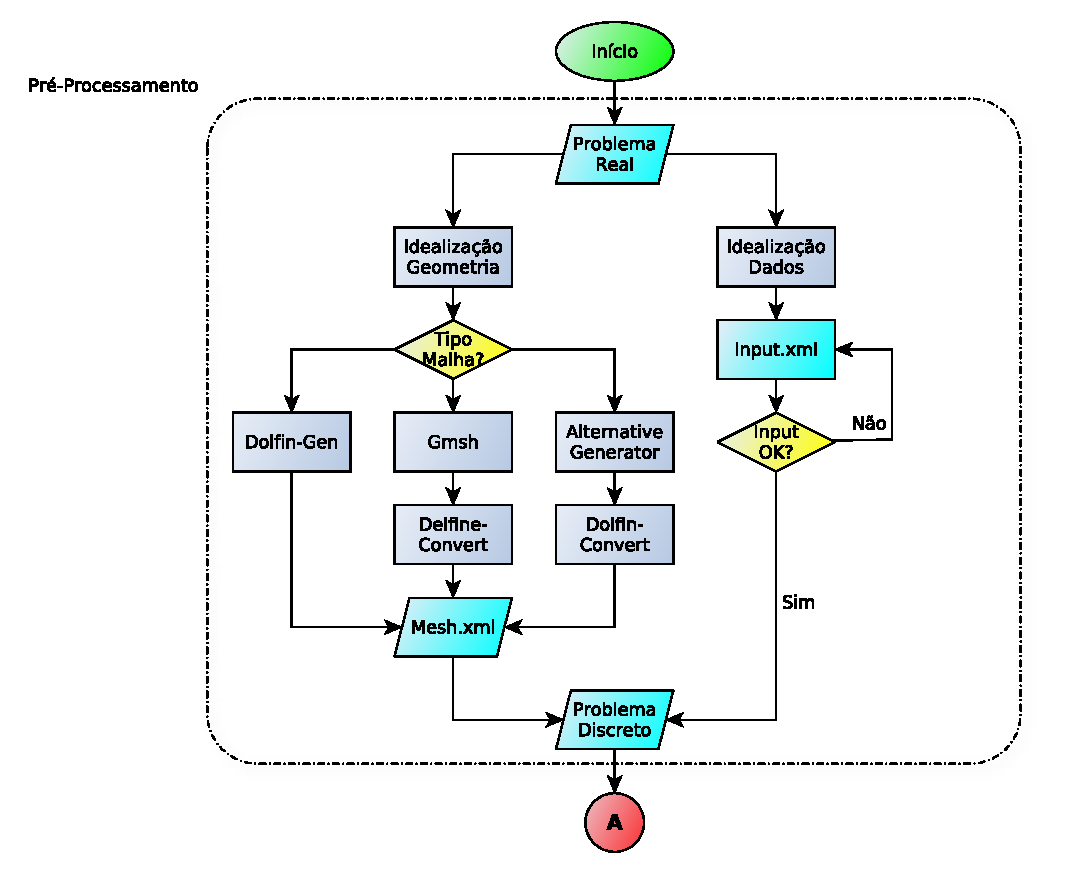
\includegraphics[width=1.0\textwidth]{chapters/ch04/Pre-Process}
\caption{Fluxograma da etapa de pr�-processamento.}
\label{fig:preprocessadorflux}
\end{figure}

\section{Processamento}
\label{sc:proc}

\begin{figure} 
\centering
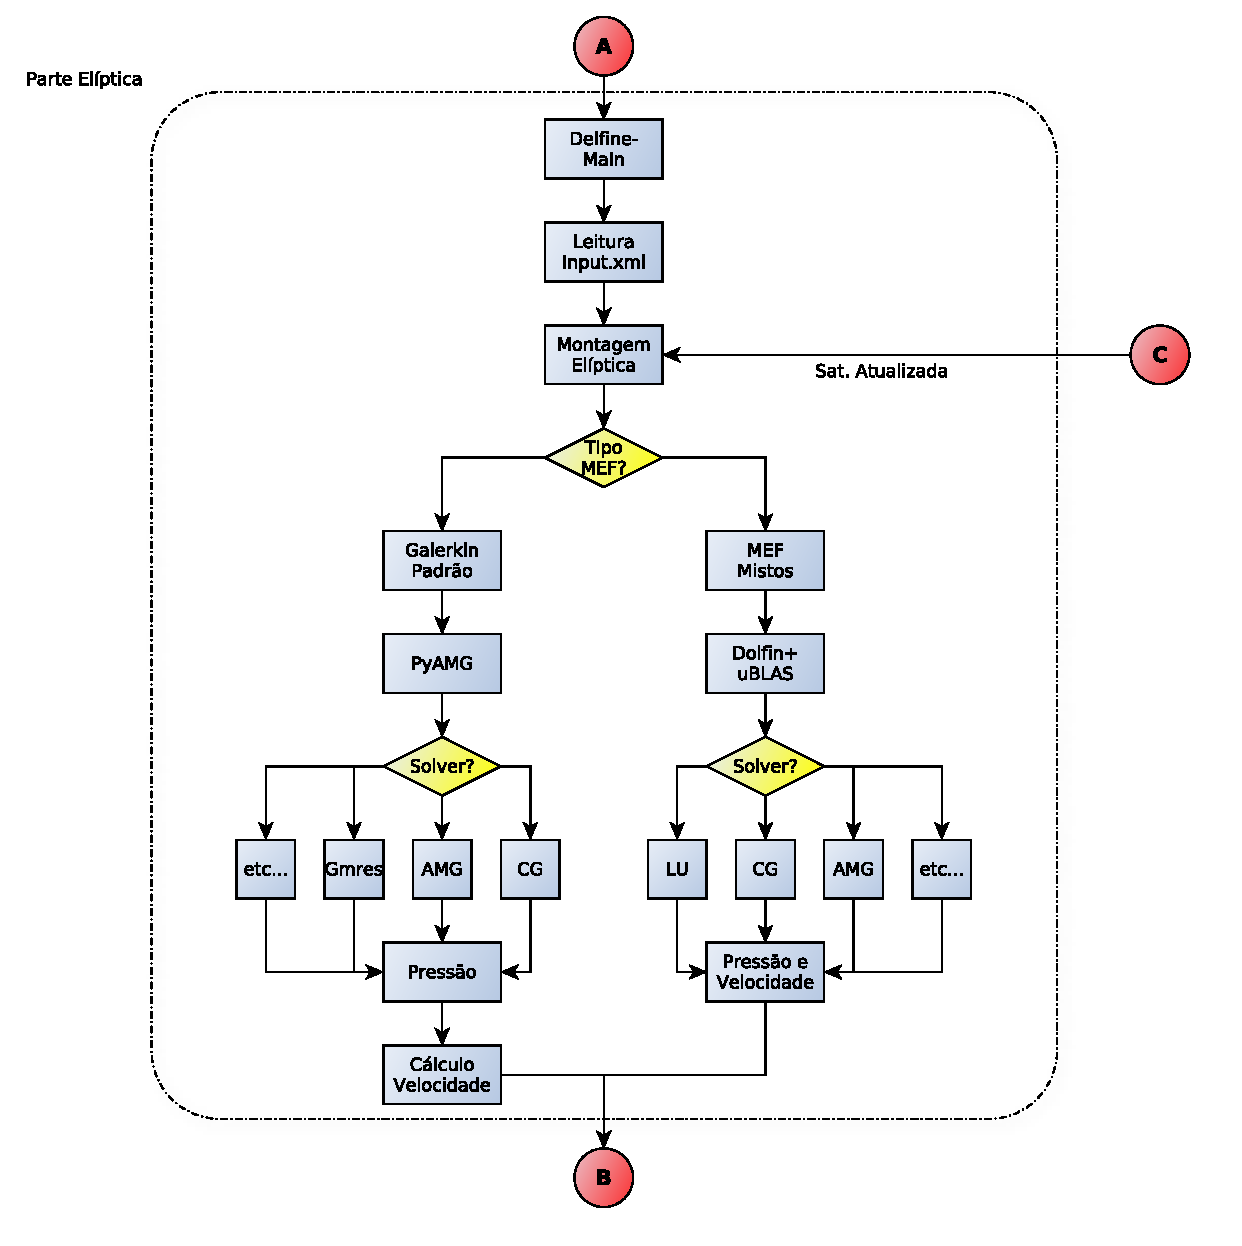
\includegraphics[width=1.0\textwidth]{chapters/ch04/Elliptic}
\caption{Fluxograma da resolu��o da parte el�ptica.}
\label{fig:ellipticflux}
\end{figure}

\begin{figure} 
\centering
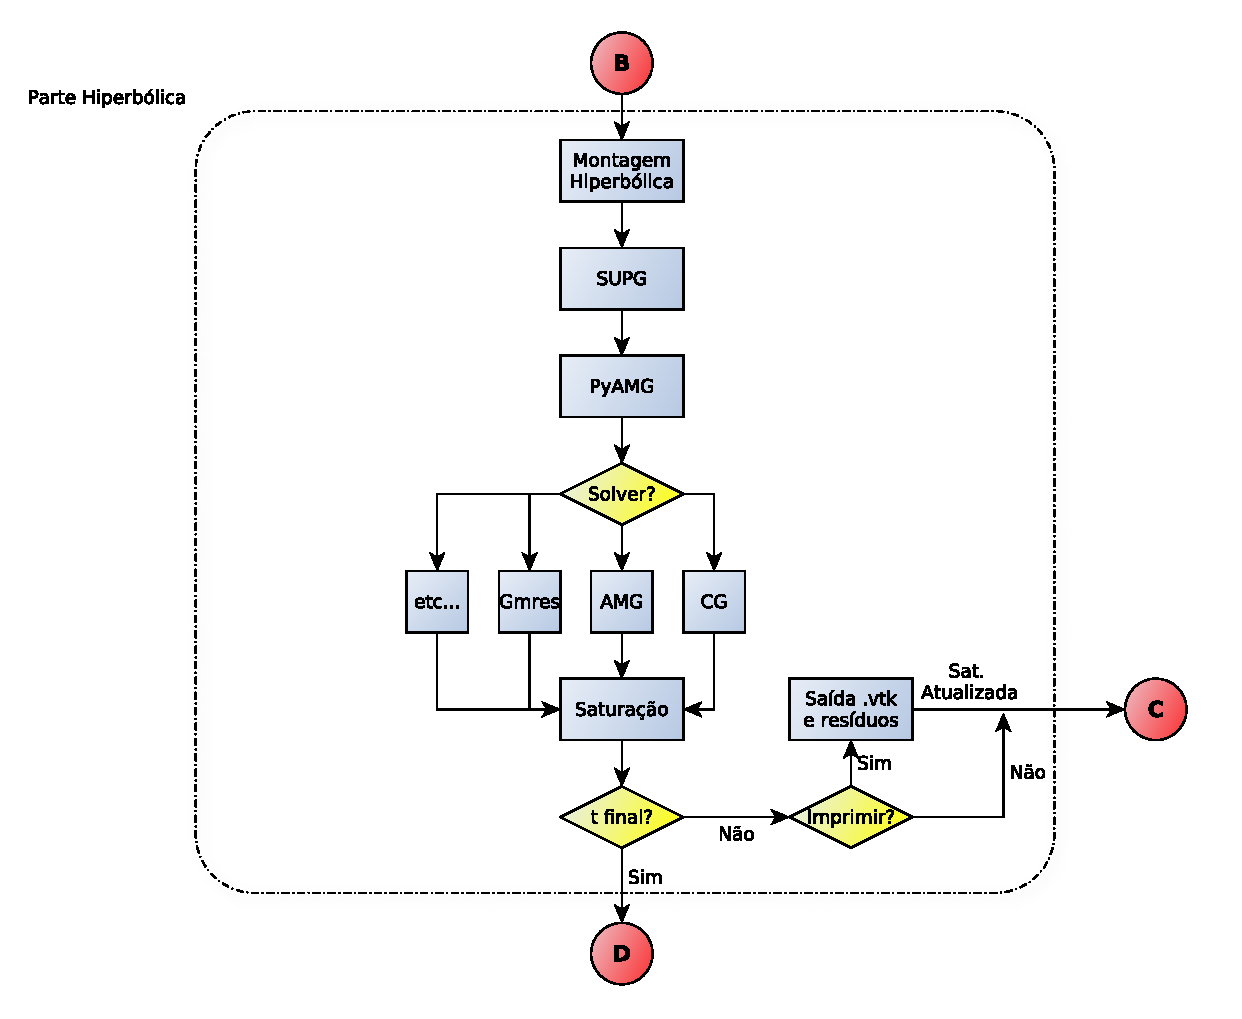
\includegraphics[width=1.0\textwidth]{chapters/ch04/Hyperbolic}
\caption{Fluxograma da resolu��o da parte hiperb�lica.}
\label{fig:hyperbolicflux}
\end{figure}

\section{P�s-Processamento}
\label{sc:pos-proc}

\begin{figure} 
\centering
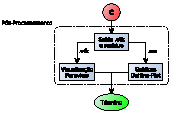
\includegraphics[width=0.7\textwidth]{chapters/ch04/Pos-Process}
\caption{Fluxograma da etapa de p�s-processamento.}
\label{fig:posprocessadorflux}
\end{figure}

% CHAPTER 05 - RESULTS
\chapter{Resultados}
\label{ch:resultados}

Neste cap�tulo ser�o apresentados exemplos e resultados obtidos utilizando a metodologia e o programa computacional descritos nos cap�tulos anteriores.

\section{Problemas El�pticos}
\label{sc:elipticos}
Esta se��o tem por objetivo avaliar os m�todos utilizados para a resolu��o da equa��o de press�o em meios porosos, a qual para o estado estacion�rio pode ser considerada uma t�pica equa��o el�ptica. Devido a essa caracter�stica, a metodologia utilizada pode ser analisada utilizando-se de problemas modelos que compartilham das mesmas propriedades matem�ticas. Uma particularidade comum aos problemas regidos por equa��es el�pticas � que todo o dom�nio de interesse $\Omega$ � afetado por qualquer mudan�a no valor da vari�vel em um ponto qualquer no interior de $\Omega$, ou em sua fronteira $\delta\Omega$ \citep{Fortuna2000}. Isto significa que uma perturba��o em um ponto ir� ter influ�ncia sobre todo o dom�nio, sendo que a mesma diminui com o aumento da dist�ncia em rela��o ao ponto originador de tal perturba��o. Sendo assim, tais problemas tendem a apresentar solu��es suaves ao longo do dom�nio. Al�m da equa��o de press�o, outros exemplos de aplica��o deste tipo de equa��o s�o o c�lculo do potencial el�trico, da difus�o de calor em uma chapa met�lica e de escoamentos incompress�veis, inv�scidos e irrotacionais (tamb�m conhecidos como escoamentos potenciais).

A equa��o de Poisson � normalmente utilizada como modelo para testar metodologias de resolu��o de equa��es el�pticas. A mesma pode ser descrita como:
\begin{equation} \label{eq:poi}
\nabla^{2} u = f
\end{equation}

Em coordenadas cartesianas e considerando um coeficiente anisotr�pico e vari�vel no espa�o $\mathbf{K}(x,y,z)$, esta equa��o pode ser representada por:
\begin{equation} \label{eq:poicart}
\frac{\partial }{\partial x}\left(\mathbf{K}\frac{\partial u}{\partial x}\right) + \frac{\partial }{\partial y}\left(\mathbf{K}\frac{\partial u}{\partial y}\right) + \frac{\partial }{\partial z}\left(\mathbf{K}\frac{\partial u}{\partial z}\right) = f(x,y,z)
\end{equation}

Nas se��es seguintes, iremos resolver equa��es do tipo \ref{eq:poicart} considerando diversas possibilidades para o coeficiente $\mathbf{K}$ de modo a demonstrar a flexibilidade da metodologia utilizada para lidar com meios homog�neos, heterog�neos, iso- e anisotr�picos. V�rios par�metros de interesse ser�o avaliados a partir dos resultados obtidos, entre eles:
\begin{itemize}
\item Erro da solu��o num�rica quando comparada com a solu��o anal�tica, a qual para problemas simples � facilmente encontrada.
\item Taxas de converg�ncias para uma sequ�ncia de malhas sucessivamente refinadas.
\item Evolu��o do res�duo para diferentes estrat�gias de resolu��o do sistema de equa��es lineares.
\end{itemize}

\subsection{Meio Homog�neo e Isotr�pico}
\label{sc:homogeneoiso}
Este primeiro exemplo foi originalmente proposto em \citep{Chen2006}, sendo resolvido utilizando dois m�todos diferentes, o CVFA (\emph{Control Volume Function Approximation}) e o CVFE (\emph{Control Volume Finite Element}). Este problema tamb�m foi explorado em \citep{Silva2008} utilizando duas varia��es do M�todo dos Volumes Finitos baseado em Arestas (EBFV1 e EBFV2). Este exemplo � um problema de valor de contorno que pode ser representado do modo a seguir:
\begin{equation} \label{eq:homogeneoiso}
\nabla(\mathbf{K} \nabla u) = 2 \pi^{2} \cos (\pi x) cos(\pi y) \quad \textrm{em  } \quad \Omega = \{(x,y) \ \vert \ 0 < x < 1 \textrm{ e } 0 < y < 1\}
\end{equation}

Onde $\mathbf{K}$ � uma matriz sim�trica e diagonal representada por:
\begin{equation} \label{eq:coeffhomoiso}
\mathbf{K} = \left( \begin{array}{cc}
1 & 0 \\
0 & 1
\end{array} \right)
\end{equation}

Este problema apresenta condi��es de contorno peri�dicas nas fronteiras inferior e superior, j� as fronteiras laterais est�o sujeitas a uma condi��o de fluxo zero. Matematicamente tais condi��es de contorno podem ser definidas do seguinte modo:
\begin{equation} \label{bchomoiso}
\left. \begin{array}{lll}
u = \cos(\pi x)  & \textrm{para } 0<x<1  \textrm{ e } y=0} \\
u = -\cos(\pi x) & \textrm{para } 0<x<1 \textrm{ e } y=1}  \\
\nabla u \cdot \vec{n} = 0 & \textrm{para } 0<y<1 \textrm{ e } x=0,1}
\end{array} \right.
\end{equation}

Resolvemos o problema el�ptico descrito utilizando a formula��o detalhada no cap�tulo \ref{ch:form_num}, considerando diferentes malhas sucessivamente refinadas e formadas por elementos triangulares de 1� e 2� ordem. Para avalia��o da acur�cia do m�todo utilizado, os resultados foram comparados com a solu��o anal�tica deste problema,a qual � representada pela fun��o $u(x,y) = \cos(\pi x)\cos(\pi y)$. A figura \ref{fig:HomogeneoIsotropico_N=64} mostra o campo escalar $u$ obtido para a malha de 64x64 elementos, a qual j� permite obter uma excelente concord�ncia com a solu��o anal�tica.

\begin{figure}
\centering
\includegraphics[width=0.5\textwidth]{chapters/ch05/HomogeneoIsotropico_N=64}
\caption[Caso homog�neo e isotr�pico. Campo escalar para malha 64x64]{Campo escalar obtido utilizando o MEF com malha de 64x64 discretizada por tri�ngulos lineares.}
\label{fig:HomogeneoIsotropico_N=64}
\end{figure}

Para uma sequ�ncia de malhas formadas por tri�ngulos lineares, se espera uma taxa de converg�ncia de segunda ordem, enquanto para uma sequ�ncia formada por tri�ngulos quadr�ticos espera-se uma converg�ncia de terceira ordem \citep{Hughes2000}. De modo a verificar o comportamento do m�todo utilizado, resolvemos o problema proposto utilizando elementos de 1�(tabela \ref{tab:homoisolinear}) e 2� ordem(tabela \ref{tab:homoisoquad}), comparando entre si os resultados obtidos e tamb�m com outros dispon�veis na literatura para elementos lineares (tabelas \ref{tab:homoisoCVFA} e \ref{tab:homoisoEBFV1}) \citep{Chen2006}\citep{Silva2008}. De um modo geral, as taxas de converg�ncias obtidas se aproximaram bastante das taxas te�ricas tanto para o caso de elementos triangulares quanto quadr�ticos. A compara��o com os resultados da literatura ficam um pouco prejudicadas por terem os erros sido calculados atrav�s de normas diferentes (norma do m�ximo neste trabalho, e RMS na literatura citada). Por�m, � poss�vel observar um comportamento coerente do erro obtido, pois com elementos quadr�ticos foram obtidos erros consideravelmente menores do que com os m�todos de segunda ordem CVFA e EBFV1. Por outro lado, ao utilizar-se elementos lineares foram obtidos erros maiores por�m na mesma ordem de grandeza daqueles obtidos na literatura.

\begin{table}
\caption[Erro e taxa de converg�ncia para problema homog�neo e isotr�pico]{Erro e taxa de converg�ncia obtidos neste trabalho para a solu��o da equa��o el�ptica em meio homog�neo e isotr�pico.} 
\centering
\subtable[Tri�ngulo Linear]{
	\begin{tabular}{|c|c|c|}
	\hline N & \vert\vert E_{max}\vert\vert & q_{max} \\
	\hline
	\hline 8 & 2.5e-02 & --- \\ 
	\hline 16 & 6.4e-03 & 1.97 \\ 
	\hline 32 & 1.6e-03 & 1.99 \\ 
	\hline 64 & 4.0e-04 & 1.99 \\ 
	\hline 128 & 1.0e-04 & 2.00 \\ 
	\hline 256 & 2.5e-05 & 1.99 \\ 
	\hline 
	\end{tabular}
	\label {tab:homoisolinear}
}
\qquad\qquad
\subtable[Tri�ngulo Quadr�tico]{
	\begin{tabular}{|c|c|c|}
	\hline N & \vert\vert E_{max}\vert\vert & q_{max} \\
	\hline
	\hline 8 & 6.4e-04 & --- \\ 
	\hline 16 & 8.7e-05 & 2.87 \\ 
	\hline 32 & 1.1e-05 & 2.94 \\ 
	\hline 64 & 1.4e-06 & 2.98 \\ 
	\hline 128 & 1.8e-07 & 2.98 \\ 
	\hline 256 & 2.2e-08 & 3.00 \\ 
	\hline 
	\end{tabular}
	\label {tab:homoisoquad}
}
\end{table}

\begin{table}
\caption[Erro e taxa de converg�ncia para problema homog�neo e isotr�pico - literatura]{Erro e taxa de converg�ncia obtidos em \cite{Chen2006} e \cite{Silva2008} para a solu��o da equa��o el�ptica em meio homog�neo e isotr�pico.} 
\centering
\subtable[CVFA\citep{Chen2006}]{
	\begin{tabular}{|c|c|c|}
	\hline N & \vert\vert E_{rms}\vert\vert & q_{rms} \\
	\hline
	\hline 8 & 1.2e-02 & --- \\ 
	\hline 16 & 3.0e-03 & 2.02 \\ 
	\hline 32 & 7.4e-03 & 2.01 \\ 
	\hline 64 & 1.8e-04 & 2.00 \\ 
	\hline 
	\end{tabular}
	\label {tab:homoisoCVFA}
}
\qquad\qquad
\subtable[EBFV1\citep{Silva2008}]{
	\begin{tabular}{|c|c|c|}
	\hline N & \vert\vert E_{rms}\vert\vert & q_{rms} \\
	\hline
	\hline 8 & 6.9-03 & --- \\ 
	\hline 16 & 1.4e-03 & 2.29 \\ 
	\hline 32 & 3.2e-04 & 2.13 \\ 
	\hline 64 & 7.7e-05 & 2.06 \\ 
	\hline 
	\end{tabular}
	\label {tab:homoisoEBFV1}
}
\end{table}

Para a resolu��o do sistema de equa��es lineares provenientes da discretiza��o do problema foram testadas tr�s diferentes alternativas:
\begin{itemize}
\item M�todos dos Gradientes Conjugados(CG) aplicado isoladamente.
\item M�todo do Multigrid Alg�brico(AMG) aplicado isoladamente.
\item Multigrid Alg�brico aplicado como pr�-condicionador para o m�todo dos Gradientes Conjugados (AMG+CG).
\end{itemize}

Para a realiza��o dos testes, foi utilizada uma malha de 32x32 elementos triangulares de 1� ordem. Para todos os casos foi considerada como crit�rio de parada uma toler�ncia $\epsilon = 10^{-10}$, com um n�mero m�ximo de 200 itera��es. Para os casos nos quais o m�todo AMG foi utilizado como forma de acelerar a converg�ncia, considerou-se ciclos do tipo $V$ em uma hierarquia de 4 "malhas" sucessivamente mais grosseiras . � importante apenas lembrar que o m�todo AMG n�o depende de malhas grosseiras propriamente ditas, apenas das matrizes que representam o sistema de equa��es, sendo tais matrizes manipuladas algebricamente de modo a se obter os n�veis mais grosseiros \citep{Trottenberg2001}. 

Como pode ser observado na figura \ref{fig:residualHomogeneoIsotropico_N=32}, os esquemas utilizando o m�todo multigrid (AMG e AMG+CG) apresentaram resultados bastante superiores em rela��o ao m�todo puramente iterativo CG. Enquanto o m�todo AMG+CG reduz o res�duo em aproximadamente uma ordem de grandeza por itera��o, o m�todo CG necessita de aproximadamente 10 vezes mais itera��es para reduzir o res�duo na mesma propor��o. � interessante comparar tamb�m os resultados obtidos ao utilizar-se o AMG isoladamente e ao us�-lo como um pr�-condicionador para o m�todo dos Gradientes Conjugados. Percebe-se que nas primeiras itera��es os dois m�todos apresentam fatores de converg�ncia para o res�duo praticamente id�nticos, por�m a medida que se prossegue com as itera��es, o AMG usado isoladamente tende a apresentar uma piora na taxa de converg�ncia, enquanto o m�todo que utiliza a combina��o AMG+CG mant�m o excelente fator de converg�ncia obtido inicialmente.

Isto se deve a um aspecto bastante observado na literatura \citep{Mavriplis2001}\citep{Trottenberg2001}\citep{Oosterlee1998} no qual um �nico ou poucos autovalores da matriz representante do operador de itera��o Multigrid est�o com um valor muito acima daquele obtido para os demais autovalores. Sendo que o autovalor m�ximo (tamb�m chamados de raio espectral) do operador de itera��o indicam em �ltima an�lise o fator de converg�ncia assimpt�tica para o problema \citep{Briggs2000}, limitando portanto a taxa de converg�ncia poss�vel de ser obtida. Um modo de contornar tal problema � justamento utilizar algum m�todo de subespa�o de Krylov, como � o caso do m�todo CG, os quais tem a caracter�stica de em poucas itera��es obter os autovetores relacionados aos poucos autovalores isolados \citep{Trottenberg2001}.

\begin{figure}
\centering
\includegraphics[width=0.7\textwidth]{chapters/ch05/residualHomogeneoIsotropico_N=32}
\caption[Caso homog�neo e isotr�pico. Compara��o da evolu��o dos res�duos para malha 32x32]{Caso homog�neo e isotr�pico. Compara��o da evolu��o dos res�duos para malha 32x32 discretizada por tri�ngulos lineares.}
\label{fig:residualHomogeneoIsotropico_N=32}
\end{figure}

\subsection{Meio Homog�neo e Anisotr�pico}
\label{sc:homogeneoaniso}
Este problema foi originalmente proposto em \cite{Crumpton1995}, onde foi resolvido utilizando um m�todo de volumes finitos centrado na c�lula (FCFV), tendo tamb�m sido estudado em \cite{Carvalho2005} e \cite{Silva2008} utilizando o j� mencionado m�todo dos volumes finitos baseado em arestas (EBFV)

Neste segundo exemplo, buscamos explorar a flexibilidade da metodologia utilizada, a qual permite considerar tensores diagonais ou cheios para representar o coeficiente $\mathbf{K}$. O problema proposto pode ser descrito atrav�s da equa��o \ref{eq:homogeneoaniso} aplicada em um dom�nio $\Omega = (0,1)x(0,1)$.
\begin{equation} \label{eq:homogeneoaniso}
\nabla(\mathbf{K} \nabla u) = -2(1 + x^2 + xy + y^2)e^{xy}
\end{equation}

Onde $\mathbf{K}$ � uma matriz sim�trica e n�o-diagonal representada por:
\begin{equation} \label{eq:coeffhomoaniso}
\mathbf{K} = \left( \begin{array}{cc}
2 & 1 \\
1 & 2
\end{array} \right)
\end{equation}

A defini��o deste problema est� completa ao definir-se a condi��o de fronteira em todo o contorno $\delta\Omega$ como $u(x,y)=e^{xy}$.

Na figura \ref{fig:HomogeneoAnisotropico_N=64} pode ser observado o campo escalar para a vari�vel $u$, considerando uma discretiza��o do dom�nio $\Omega$ com uma malha de 64x64 elementos triangulares de 1� ordem.

\begin{figure}
\centering
\includegraphics[width=0.5\textwidth]{chapters/ch05/HomogeneoAnisotropico_N=64}
\caption[Caso homog�neo e anisotr�pico. Campo escalar para malha 64x64]{Caso homog�neo e anisotr�pico. Campo escalar obtido utilizando o MEF com malha de 64x64 discretizada por tri�ngulos lineares.}
\label{fig:HomogeneoAnisotropico_N=64}
\end{figure}

De modo a comparar os resultados obtidos com aqueles da literatura, calculamos o erro segundo a norma do m�ximo e as taxas de converg�ncias para o mesmo considerando uma sequ�ncia de malhas sucessivamente refinadas (ver tabela \ref{tab:homoanisolinear}). Tais resultados foram comparados com aqueles obtidos tanto pelo FCFV quanto pelo EBFV (ver tabelas \ref{tab:homoanisocrump} e \ref{tab:homoanisocarvalho}).

\begin{table}
\caption[Erro e taxa de converg�ncia para problema homog�neo e anisotr�pico]{Erro e taxa de converg�ncia obtidos neste trabalho para a solu��o da equa��o el�ptica em meio homog�neo e anisotr�pico.} 
\centering
\subtable[Tri�ngulo Linear]{
	\begin{tabular}{|c|c|c|}
	\hline N & \vert\vert E_{max}\vert\vert & q_{max} \\
	\hline
	\hline 8 & 2.1e-03 & --- \\ 
	\hline 16 & 5.3e-04 & 2.01 \\ 
	\hline 32 & 1.3e-04 & 2.00 \\ 
	\hline 64 & 3.3e-05 & 1.99 \\ 
	\hline 128 & 8.3e-06 & 2.00 \\ 
	\hline 256 & 2.1e-06 & 2.00 \\ 
	\hline 
	\end{tabular}
	\label {tab:homoanisolinear}
}
\end{table}

\begin{table}
\caption[Erro e taxa de converg�ncia obtidos na literatura para problema homog�neo e anisotr�pico]{Erro e taxa de converg�ncia obtidos em \cite{Crumpton1995} e \cite{Carvalho2005} para a solu��o da equa��o el�ptica em meio homog�neo e anisotr�pico.} 
\centering
\subtable[FCFV\citep{Crumpton1995}]{
	\begin{tabular}{|c|c|c|}
	\hline N & \vert\vert E_{rms}\vert\vert & q_{rms} \\
	\hline
	\hline 8 & 1.2e-03 & --- \\ 
	\hline 16 & 2.9e-04 & 2.00 \\ 
	\hline 32 & 7.3-05 & 1.99 \\ 
	\hline 64 & 1.8e-05 & 1.99 \\ 
	\hline 
	\end{tabular}
	\label {tab:homoanisocrump}
}
\qquad\qquad
\subtable[EBFV\citep{Carvalho2005}]{
	\begin{tabular}{|c|c|c|}
	\hline N & \vert\vert E_{max}\vert\vert & q_{max} \\
	\hline
	\hline 8 & 3.0e-03 & --- \\ 
	\hline 16 & 1.0e-03 & 1.58 \\ 
	\hline 32 & 3.4-04 & 1.80 \\ 
	\hline 64 & 8.9-05 & 1.94 \\
	\hline 
	\end{tabular}
	\label {tab:homoanisocarvalho}
}
\end{table}

Pode-se observar pelo resultados obtidos que novamente o MEF se comportou como esperado, apresentado uma taxa de converg�ncia de ordem 2 para os elementos lineares. Os valores absolutos do erro na norma do m�ximo se comparam de maneira ligeiramente favor�vel aqueles apresentado em \cite{Carvalho2005}.

Assim como para o primeiro exemplo, tamb�m neste fizemos um estudo a respeito da performance de diferentes m�todos iterativos para a resolu��o do sistema de equa��es lineares provenientes da discretiza��o do problema. Cinco diferentes alternativas foram testadas:
\begin{itemize}
\item M�todos dos Gradientes Conjugados (CG) aplicado isoladamente.
\item M�todos do Res�duo M�nimo Generalizado (GMRES) aplicado isoladamente.
\item M�todo do Multigrid Alg�brico (AMG) aplicado isoladamente.
\item Multigrid Alg�brico aplicado como pr�-condicionador para o m�todo dos Gradientes Conjugados (AMG+CG).
\item Multigrid Alg�brico aplicado como pr�-condicionador para o m�todo do Res�duo M�nimo Generalizado (AMG+GMRES).
\end{itemize}

\begin{figure}
\centering
\includegraphics[width=0.7\textwidth]{chapters/ch05/residualHomoAniso_N=64}
\caption[Caso homog�neo e anisotr�pico. Compara��o da evolu��o dos res�duos para malha 64x64]{Caso homog�neo e anisotr�pico. Compara��o da evolu��o dos res�duos para malha 64x64 discretizada por tri�ngulos lineares.}
\label{fig:residualHomogeneoAnisotropico_N=64}
\end{figure}

Para a realiza��o dos testes, foi utilizada uma malha de 64x64 elementos triangulares de 1� ordem. Para todos os casos foi considerada como crit�rio de parada uma toler�ncia $\epsilon = 10^{-10}$, com um n�mero m�ximo de 200 itera��es. Em todos os casos nos quais o m�todo AMG foi utilizado como forma de acelerar a converg�ncia, considerou-se ciclos do tipo $V$ em uma hierarquia de 4 "malhas" sucessivamente mais grosseiras. Um gr�fico mostrando a evolu��o do res�duo normalizado para todos os m�todos testados pode ser observado na figura \ref{fig:residualHomogeneoAnisotropico_N=64}, onde fica claro novamente a grande superioridade dos m�todos que utilizam acelera��o de converg�ncia via multigrid em compara��o com procedimentos puramente iterativos. � interessante notar tamb�m que para este exemplo os m�todos CG e GMRES tiveram desempenhos bastante pr�ximos, tanto isoladamente quanto em conjunto com o AMG enquanto pre-condicionador.



\subsection{Meio Heterog�neo e Anisotr�pico}
\label{sc:heterogeneoaniso}

\section{Problemas de Escoamentos Bif�sicos em Meios Porosos}
\label{sc:escoabifasico}
Ao se considerar tamb�m a equa��o de satura��o, o problema do deslocamento de fluidos em meios porosos passa a ter tamb�m um componente altamente hiperb�lico.
\subsection{1/4 de Cinco Po�os Homog�neo}
\label{sc:quarterfivespothomo}
\subsection{1/4 de Cinco Po�os Heterog�neo}
\label{sc:quarterfivespothetero}


% CHAPTER 06 - CONCLUSION
\chapter{Conclus�es e Trabalhos Futuros}
\label{ch:conclusoes}

\section{Conclus�es}
\label{sc:conclusoes}
In this work, a procedure for the solution of the pressure equation in heterogeneous and anisotropic porous media was presented. The PDEs resultant from the mathematical modeling were solved using a Standard Galerkin Finite Element Method approach. In order to accelerate the convergence of the resultant system of equations, an Algebraic Multigrid method was employed, both as stand-alone and as a preconditioner to other solvers. As this kind of numerical framework normally imply in a great time-effort in developing the computational tools that implement them, this work used some available open source libraries in order to automate the generation of low-level code based on some high-level description of the problem. This showed to be a very efficient work methodology, as it allowed to experiment more with the problem in question in less time, because the developer spares time that would be used in "administrative" coding tasks. The results obtained for a model example showed the good performance of the proposed procedure, as the solution converged even for a heterogeneous and highly anisotropic problem. 

\section{Trabalhos Futuros}
\label{sc:trabFuturos}
A future work, which is already in progress, will be the solution of the saturation equation associated with the pressure by means of the velocity. The pressure-velocity equation will be solved using a mixed FEM and the saturation equation using a Petrov-Galerkin FEM.



%%%%%%%%%%%%%%%%%%%%%%%%%%%%%%%%%%%%%%%%%%%%%%%%%%%%%%%%%%%%%%%%%%%%%%%%
%% BACK MATTER
%%%%%%%%%%%%%%%%%%%%%%%%%%%%%%%%%%%%%%%%%%%%%%%%%%%%%%%%%%%%%%%%%%%%%%%%
\bibliographystyle{natbib}
\addcontentsline{toc}{chapter}{Refer�ncias Bibliogr�ficas}

% REFERENCES
\bibliography{chapters/extras/references}

% APPENDIX
\clearpage
\appendix

% A01 - USER GUIDE
\chapter{Delfine - Manual do usu�rio}
\label{ch:manual}

Manual do us�rio do Delfine.

\section{Instala��o do Programa}
\label{sc:estrutura}
Mostrar onde o programa pode ser baixado. Descrever depend�ncias do mesmo. Focar em uma instala��o do Ubuntu. Descri��o da estrutura geral do programa.

\section{Dados de Entrada}
\label{sc:entrada}
Descri��o do arquivo .xml de entrada. Tamb�m descrever as possibilidades de gera��o de malha(gmsh com convers�o, fun��es pr�prias do dolfin, uso de arquivo .xml do dolfin convertido a partir de outros formatos utilizando o convert-mesh, etc.)

\section{Exemplo Detalhado}
\label{sc:exemplo}
Mostrar como rodar um exemplo simples utilizado na tese.




\end{document}